%!TEX root = thesis.tex
%%%%%%%%%%%%%%%%%%%%%%%
%
%
%%%%%%%%%%%%%%%%%%%%%%%%%%%%%%%%%
%%%%%%%%%%%%%%%%%%%%%%%%%%%%%%%%%
\chapter{Matrix product states}
\label{ch:matrix_product_states}
%%%%%%%%%%%%%%%%%%%%%%%%%%%%%%%%%
%%%%%%%%%%%%%%%%%%%%%%%%%%%%%%%%%
%
%
The analytical treatment presented in the previous chapter relies on a heavy line of approximations.
One of the most crucial consequence of these simplifications is that quantitative deviations occur if the interactions are comparable to the kinetic bandwidth.
This restricts heavily the validity region of the low-energy effective field theory of a particular model.
To make an example, a sine-Gordon term with $\beta=4$ is encountered in the effective low-energy field theory of the spin-$1/2$ XXZ chain and the interaction will be relevant in the RG sense for $K<1/2$.
Such a small Luttinger parameter typically requires very strong nearest neighbor interactions that are compatible with the system's bandwidth\footnote{The XXZ model is integrable and the phase transition occurs when all couplings are equal to each other.}, which thus implicitly breaks the assumptions to derive the effective low-energy field theory in the first place.
Although the field theoretic description might not break down entirely, heavy quantitative deviations from the Luttinger liquid predictions of the effective coupling parameters are to be expected.
This motivates the use of numerical tools to verify the analytic predictions in the strongly interacting cases.
In this chapter, we will provide the essentials to get acquainted with the concepts of tensor networks, in particular with matrix product states (MPS).

First, we give a basic introduction to tensor networks and explain the intuitive concept of renormalization through a truncation of the auxiliary dimension of these structures.
Second, we review the concept of ``area laws'' -- a statement about the structure of quantum correlations of gapped and short-ranged Hamiltonians -- and connect it to the properties of tensor networks.
We then present renormalization strategies which provide variational search algorithms to target ground (and low-lying excited) states and continue by presenting a simple yet effective time-evolution algorithm in the framework of MPS.
At the end of the chapter, we explain how temperature and mixed states can be encoded in the framework of MPS, and review shortly the exploit of Abelian symmetries in the numerical techniques which in general reduces the overall computational complexity.
%
%
%%%%%%%%%%%%%%%%%%%%%%%%%%%
\section{Tensor networks}
\label{sec:tensor_networks}
%%%%%%%%%%%%%%%%%%%%%%%%%%%
%
%
A tensor is a collection of complex numbers in multidimensional arrays.
Its rank is given by the number of indices: for instance, scalar values are of rank zero, vectors of rank one and matrices of rank two\footnote{
    Note that the rank of a tensor differs from the usual understanding of a rank in terms of the image space dimensions.
}.
Tensor networks are in general contractions of many tensors and as such it is customary to define graphical representations which display its fundamental structure, i.e. its rank.
The most common convention is to represent a tensor object as a circle, triangle, hourglass or rectangle with as many legs as the tensor has indices.
It is then easy to sketch the tensor contraction of a simple matrix-matrix multiplication as
\begin{align}
    C_{i,j}=A_{ik}B_{kj}\equiv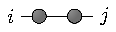
\includegraphics[valign=c]{figures/MatrixMultiplication.pdf},
\end{align}
in which we conveniently use the sum convention.
Switching from formulas to graphical notation may become interesting when considering larger tensor networks.
One easy example is a trace of many matrices, which can be sketched as a circle contraction.
\begin{align}
    \tr\brlr{ABCDEF} \equiv 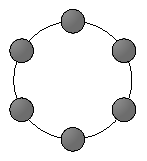
\includegraphics[valign=c]{figures/MatrixTrace.pdf}.
\end{align}
For more complex contractions containing tensors of higher ranks, it is important to optimize the sequence of contractions to reduce the overall computational cost to a minimum.
For instance, in \cref{fig:contraction_sequences} two different sequences of contractions obviously result in the same outcome, but the overall complexity class is different.
Assume each leg has dimension $m$, then sequence $S_1$ is $O(m^4)$ whereas sequence $S_2$ is $O(m^5)$.
\begin{figure}
    \centering
    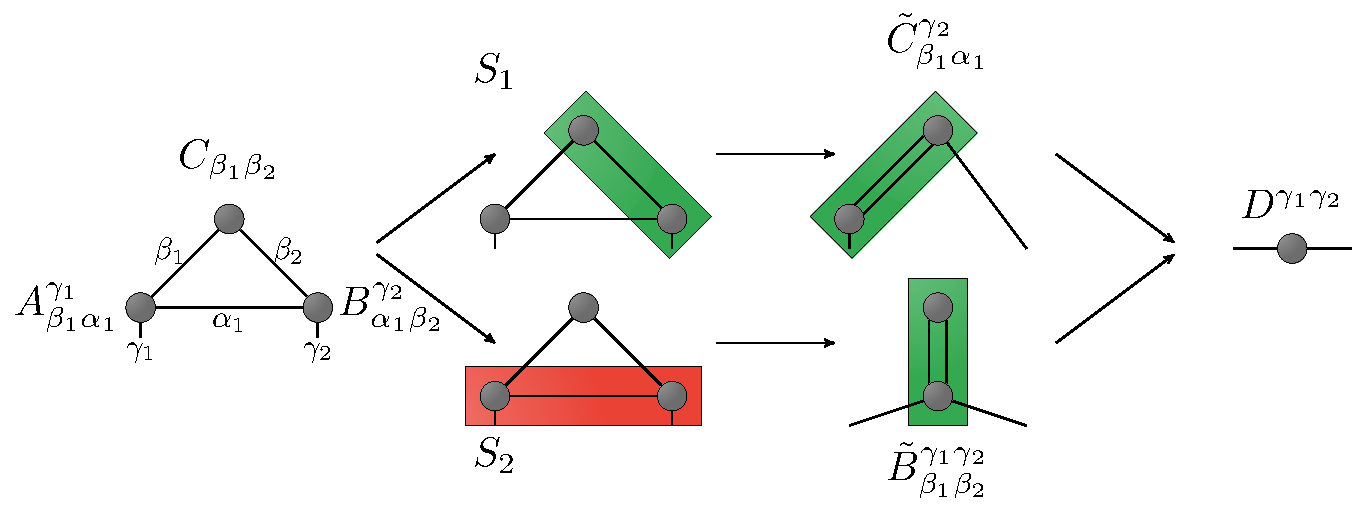
\includegraphics[width=0.8\textwidth]{figures/ComplexContraction1.pdf}
    \caption{Different complexity classes for the same contraction, but different sequences. Assume each index has dimension $m$, then the green contractions are $O(m^4)$, but red is $O(m^5)$. Hence, sequence $1$ requires less multiplications compared to $2$ and is thus less prone to numerical truncation errors.}
    \label{fig:contraction_sequences}
\end{figure}

A triangle representation may make sense to indicate a tensor being an isometry.
For instance, consider the two isometries $U$, $V^\dag$ of a generic singular value decomposition (SVD) $M = U \Lambda V^\dag$: they contain the left- and right-singular vectors of $M$ and are thus semi-unitaries, i.e.
\begin{align}
    U^\dag U^\pdag = \mathbb1,
    \quad
    V^\dag V^\pdag = \mathbb1.
\end{align}
In graphical notation, the identity matrix is represented as a straight line as it does neither stretch nor rotate the entries of a tensor.
The previous equation can thus be recast to
\begin{align}
    U^\dag U^\pdag \equiv 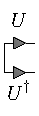
\includegraphics[valign=c]{figures/right_isometry.pdf} = 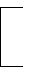
\includegraphics[valign=c]{figures/right_identity.pdf}\,,
    \qquad
    V^\dag V^\pdag \equiv 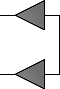
\includegraphics[valign=c]{figures/left_isometry.pdf} = 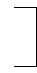
\includegraphics[valign=c]{figures/left_identity.pdf}\,.
    \label{eq:isometries}
\end{align}
Although the two pictures represent the same multiplication at the present stage, a distinction of the two will be useful in the context of canonical MPS at a later point (in particular, in \cref{eq:isometry_tensors_diagram}).
A simple squared unitary matrix is orthogonal with respect to both left/right multiplication with its adjoint and as such can be represented as a hourglass.
The SVD of a normal matrix $M$ can be recast to the graphical notation
\begin{align}
    
\includegraphics[valign=c]{figures/matrix.pdf}
    \equiv M = U \Lambda V^\dag \equiv
    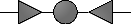
\includegraphics[valign=c]{figures/svd.pdf}\,.
\end{align}
Let me now introduce probably the most important decomposition applied in tensor networks -- the generalized version of the SVD for rank $n$ tensors\footnote{For tensor network experts, do not confuse with the higher order SVD (HOSVD) or Tucker decomposition.}:
(i) the rank $n$ array has to be reduced to a rank $2$ object, i.e. a matrix.
This transformation (which must be a bijection) is commonly called tensor reshaping and is understood in graphical notation as a fusion of multiple tensor legs.
(ii) The matrix then is decomposed through a standard SVD, followed by (iii) the restoration of the original rank $n$ object through the inverse reshaping applied in step (i).
The identity relation between the original and decomposed tensor is assured by the inverse of (i).
For a practical example, consider a rank $n$ tensor $T$ which is graphically depicted by $n$ legs (labelled by increasing numbers from $1,...,n$ from left to right).
To perform a SVD between the bipartition after leg $j$, the tensor is reshaped to a matrix through a fusion of legs $1,...,j$ and $j+1,...,n$ prior to the performed SVD, after which the original rank is restored.
In particular, the sequence of identities reads
% \begin{align}
%     % 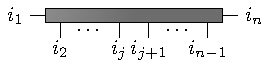
\includegraphics[valign=c]{figures/rankntensor.pdf}
%     % =
%     T_{i_1,i_n}^{i_2,\dots,i_j,i_{j+1},\dots,i_{n-1}}
%     &\overset{(i)}{=}
%     f^{-1}\circ T_{(i_1,\dots,i_j),(i_{j+1},\dots,i_n)}
%     \\
%     &\overset{(ii)}{=}
%     f^{-1}\circ\sum_k U^\pdag_{(i_1,\dots,i_j),k}S^\pdag_{k}{V^\dag}_{k,(i_{j+1},\dots,i_n)}
%     \\
%     &\overset{(iii)}{=}
%     \sum_kU_{i_1,k}^{i_2,\dots,i_j}S^\pdag_{k}{V^\dag}_{k,i_n}^{i_{j+1},\dots,i_{n-1}},
% \end{align}
\begin{align}
    T_{i_1,i_n}^{i_2,\dots,i_j,i_{j+1},\dots,i_{n-1}}
    \equiv&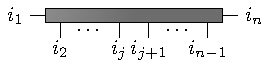
\includegraphics[valign=c]{figures/rankntensor.pdf},
    \\
    \overset{(i)}{=}&
    f^{-1}\circ
    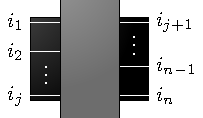
\includegraphics[valign=c]{figures/reshaping.pdf}
    \equiv
    f^{-1}\circ U^\pdag_{(i_1,\dots,i_j),k}\Lambda^\pdag_{k}V^\dag_{k,(i_{j+1},\dots,i_n)},
    \\
    \overset{(ii)}{=}&
    f^{-1}\circ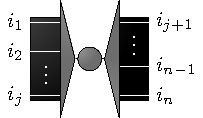
\includegraphics[valign=c]{figures/bigsvd.pdf}
    \equiv
    f^{-1}\circ U^\pdag_{(i_1,\dots,i_j),k}\Lambda^\pdag_{k}V^\dag_{k,(i_{j+1},\dots,i_n)},
    \\
    \overset{(iii)}{=}&
    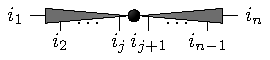
\includegraphics[valign=c]{figures/rankntensor_decomposed.pdf}
    \equiv
    U_{i_1,k}^{\pdag i_2,\dots,i_j}\Lambda^\pdag_{k}{V^\dag}^{i_{j+1},\dots,i_{n-1}}_{k,i_n},
    \label{eq:SVD_generalized}
\end{align}
in which $f^{-1}$ denotes the inverse of the tensor reshaping / leg fusion, and Einstein notation implies the tensor contraction contraction with summed index $k$.
In the equations above, it is assumed that the applied SVD is compact: $\Lambda$ is a square and diagonal matrix containing the nonzero singular values, such that $\Lambda_{ij}\equiv s_i\delta_{ij}$.

To get acquainted with the use of tensors in a more practical sense, let us aim to understand some of the described concepts in the context of two-dimensional pictures.
If we assume the picture to be rasterized in an equidistant manner using square pixels, the RGB-entries of the pixel can be collected in a 3D array of the form
\begin{align}
    P_{y,x}^{c}\equiv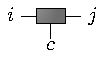
\includegraphics[valign=c]{figures/tensor_picture.pdf}.
\end{align}
The position of the pixel is encoded by the indices $y,x$ and $c$ represents a leg containing the RGB-values (e.g., $c\in\{1,2,3\}\equiv\{r,g,b\}$).
Using the concept of the generalized SVD, we can decompose the tensor $P$ into two semi-unitaries $U,V^\dag$ and a vector $S_k$ containing the singular values of the bipartition.
There exist three different bipartitions: (a) $P_{(y,x),c}$, (b) $P_{(y,c),x}$ and (c) $P_{y,(x,c)}$.
(b) and (c) are equivalent up to a transposition of the original object, therefore leaving two truly different decompositions, (a) and (b).
The bipartition (a) targets a decomposition between $(y,x)$ and $c$ whereas (b) targets a decomposition between $y$ and $(x,c)$.
Strategy (a) thus aims to truncate the color degree of freedom, which is not very useful due to the low dimensionality of the $c$ leg (there are only $3$ nonzero singular values to begin with), such that we will focus entirely on the decomposition of (b).

\begin{figure}
    \centering
    \subfigure[]{
\includegraphics{figures/SVD_uncompressed.png}}
    \hfil
    \subfigure[]{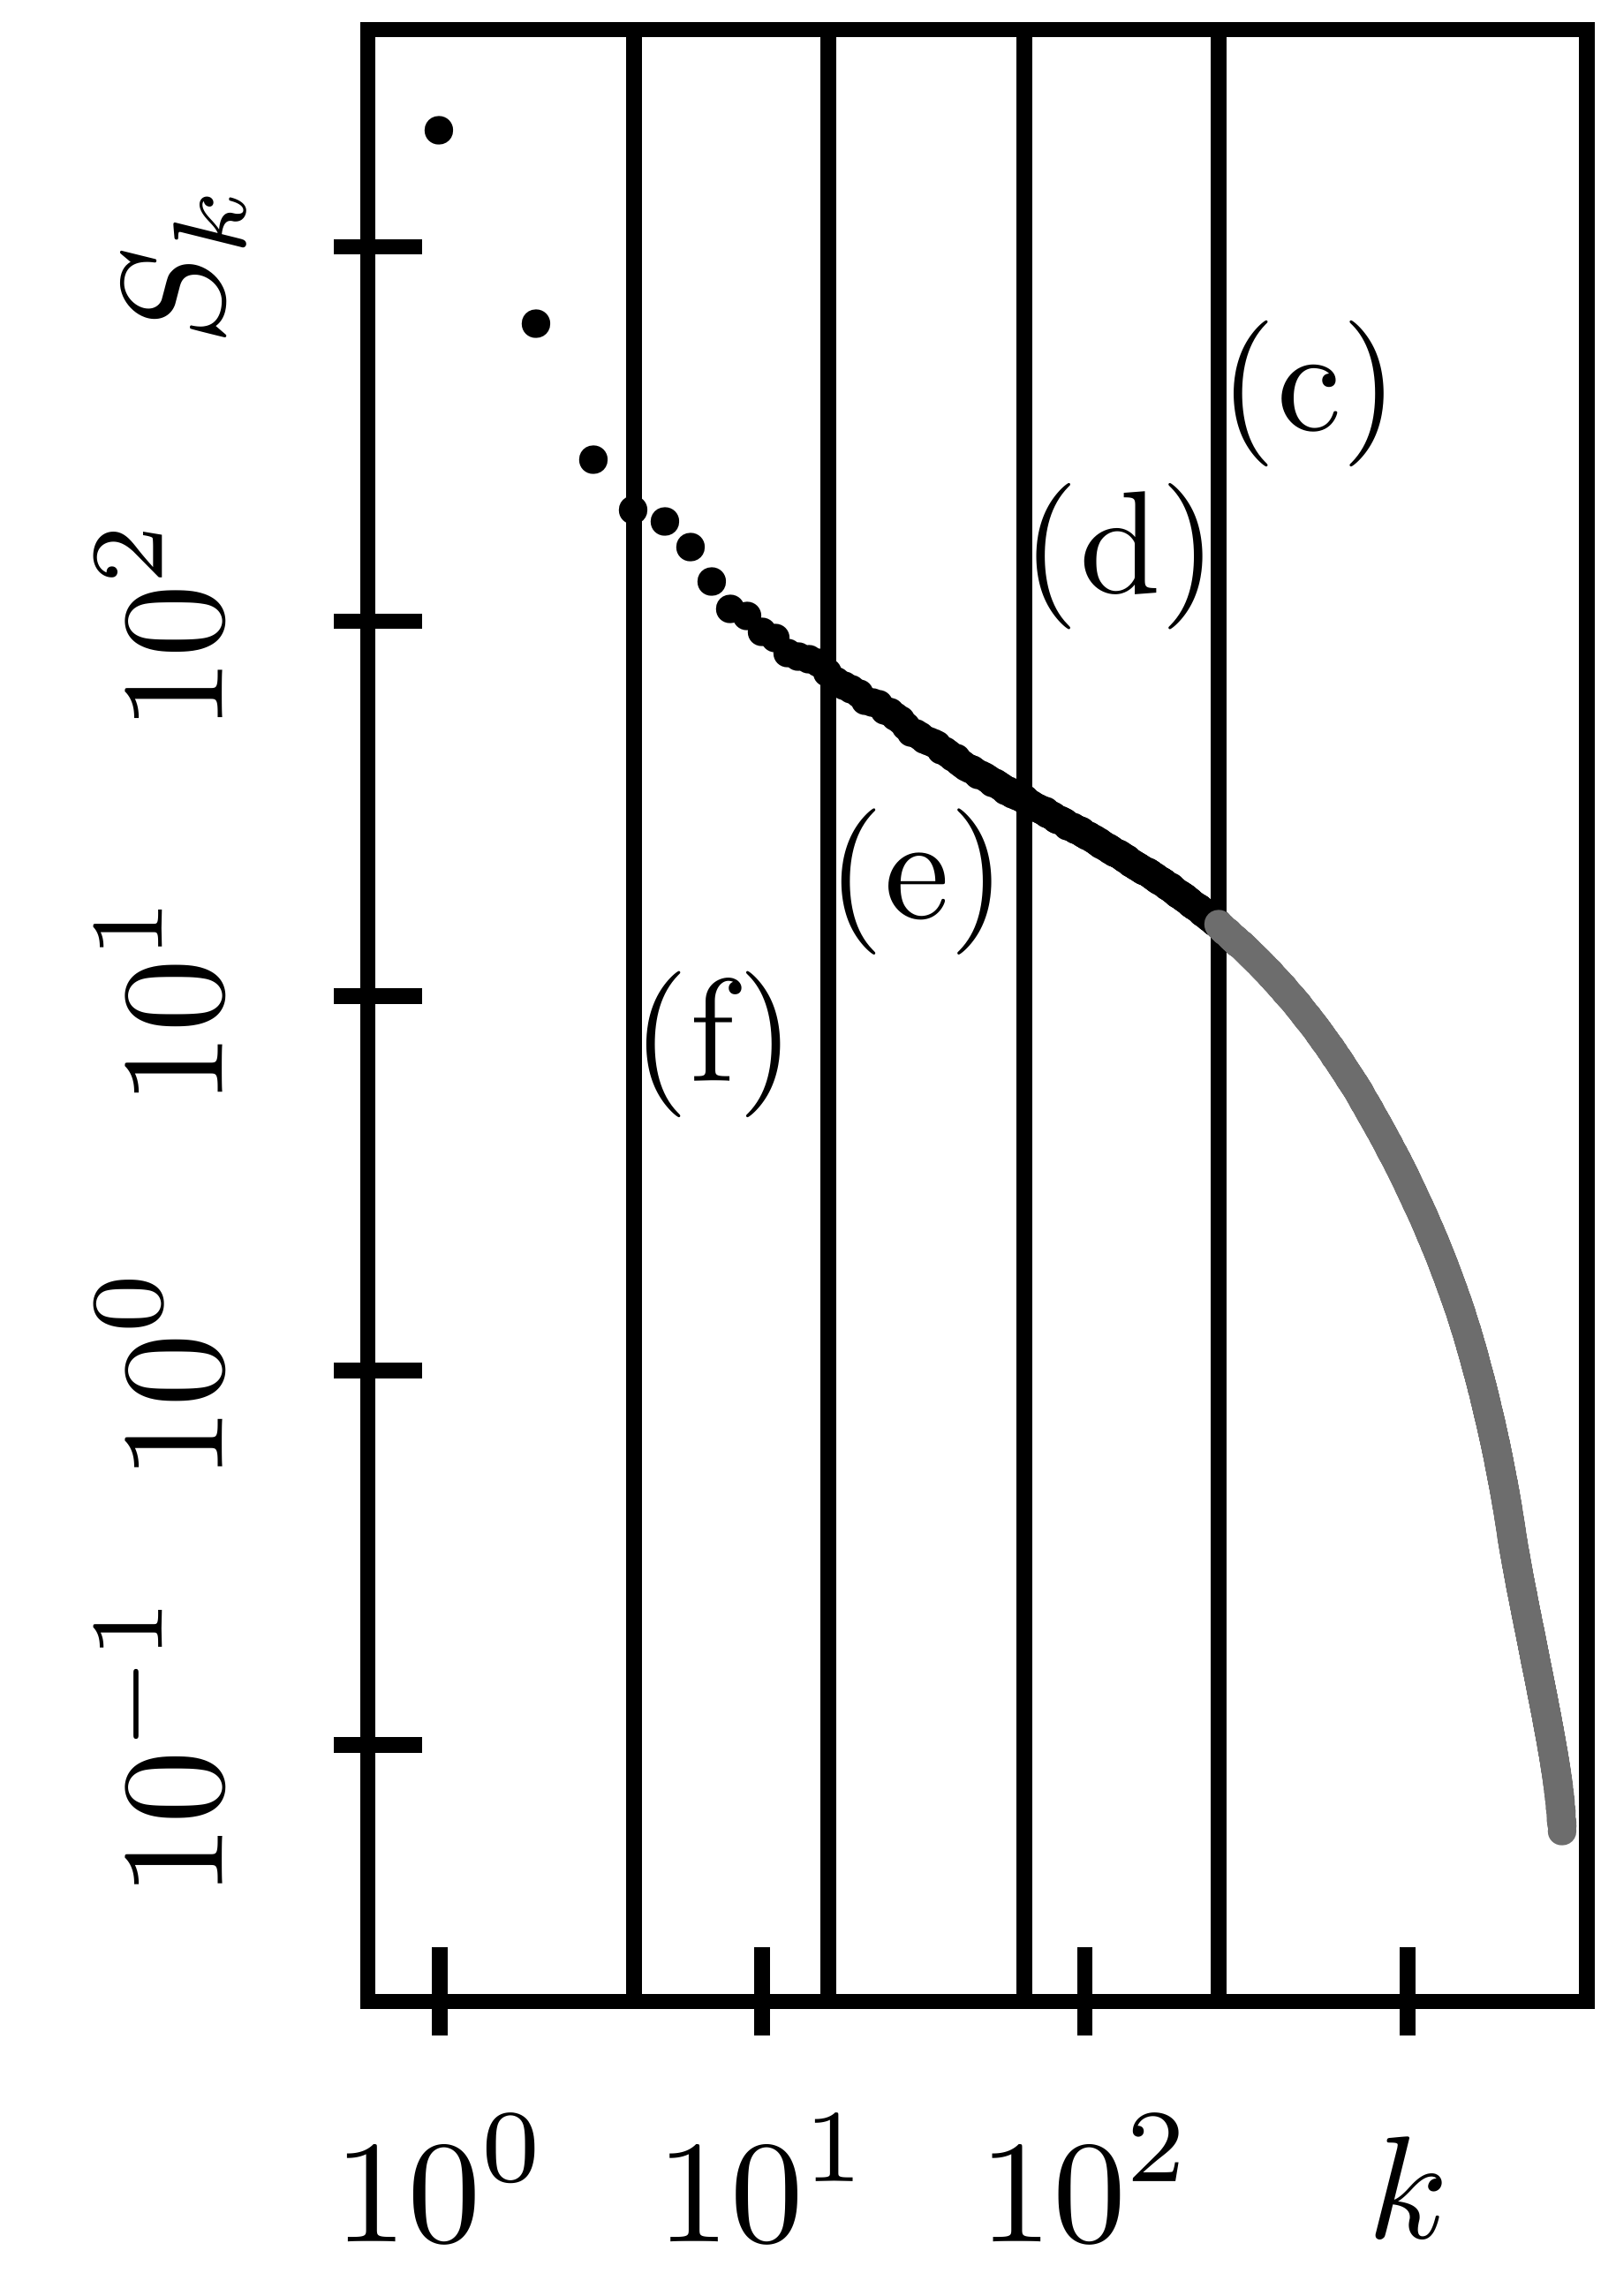
\includegraphics{figures/beach_singular_values.png}}
    \hfil
    \subfigure[]{
\includegraphics{figures/SVD_compressed.png}}
    \hfil
    \subfigure[]{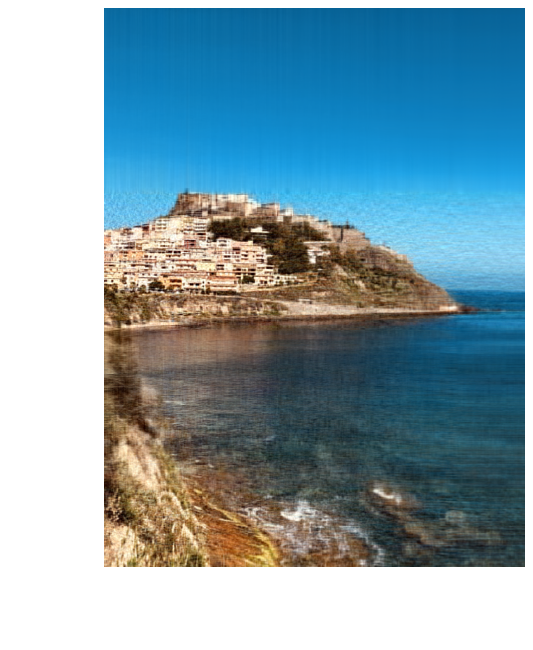
\includegraphics{figures/SVD_compressed2.png}}
    \hfil
    \subfigure[]{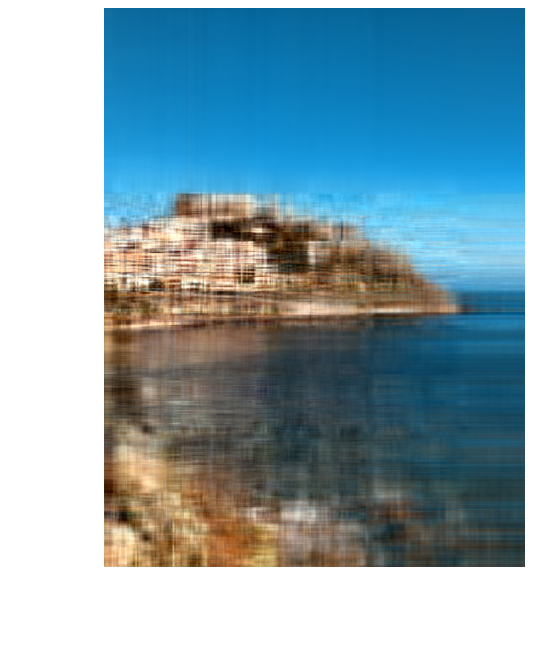
\includegraphics{figures/SVD_compressed3.png}}
    \hfil
    \subfigure[]{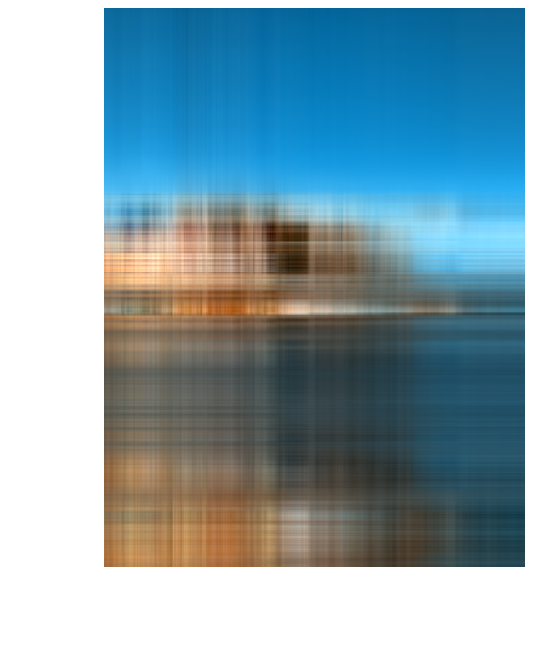
\includegraphics{figures/SVD_compressed4.png}}
    \caption{(a) Uncompressed picture of Castelsardo (Sardinia, IT).
    The digital picture consists of $n_y\times n_x=3024\times2276$ pixels. (b) Singular values of the matrix $P_{i,(jc)}$ representing the picture. (c) Keeping the $m\equiv260$ largest singular values still yields a good approximation of the uncompressed picture and requires only $20\%$ of the original storage space. Panels (d)-(f) visualize the impact of progressively lowering $m$ (later we will call this quantity the ``bond dimension''): while details are still visible in picture (d), they gradually disappear in panel (e) until even the dominant shapes become unrecognizable in figure (f).}
    \label{fig:svd_image_compression}
\end{figure}
If the singular/spectral values are ordered, a truncation of the $\Lambda$ matrix neglects subdominant left and right eigenvectors of the original object and as such approximates the original matrix.
In case of a subsequent normalization to the original trace, the truncation process can be understood as a compression or tensor renormalization scheme.
The number of singular values kept in the approximation is thus naturally linked to the accuracy of the numerical renormalization.
Assume the picture to be of dimensions $\dim(P)=p_y\times p_x\times 3$, then keeping $m$ singular values implies that we need to store only a fraction of the matrices $U$ and $V^\dag$ to approximate the original picture $P$.
Assuming that the matrix $M\equiv \{P_{y,(x,c)}\}_{y,x,c}$ is of dimension $n_y=p_y$ times $n_x=3p_x$, the following visualization highlights the SVD
\begin{align}
    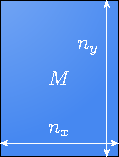
\includegraphics[valign=c]{figures/svd_mmat.pdf}
    =
    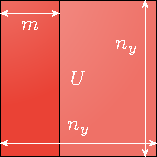
\includegraphics[valign=c]{figures/svd_umat.pdf}
    \
    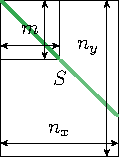
\includegraphics[valign=c]{figures/svd_smat.pdf}
    \
    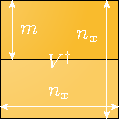
\includegraphics[valign=c]{figures/svd_vmat.pdf}.
    \label{eq:compression_scheme}
\end{align}
If we limit to $m$ spectral values, we only need to store $n_y\cdot m$ elements from $U$, $m$ singular values and $m\cdot n_x$ elements from $V^\dag$.
In total, we thus arrive at a compression rate
\begin{align}
    C_m = \frac{(n_x+n_y+1)m}{n_x n_y},
\end{align}
which allows for a high compression in case of a large and dense matrix $M$.
To give an example, we present the impact of compression in \cref{fig:svd_image_compression}.
Panel (a) denotes an uncompressed picture, the singular values of the digital picture presented in (b), and the result of keeping $m=260$ singular values as an approximation to the full picture, presented in (c).
The impact of gradually decreasing the value of $m$ is visualized in panels (d) - (f).

In a second example, we consider a fraction of the Mandelbrot set embedded in Gaussian noise presented in \cref{fig:svd_image_compression_mandelbrot}.
The visualization aims to compare the original picture for different levels of noise (panels (b) and (d-f)) with the approximation (panels (c) and (g-i)) in which the 100 smallest Schmidt values are kept (indicated by the black grid line in panel (a)).
The distribution of the spectral values is controlled by the fraction of random noise mixed into the picture: the decay is weaker for a larger fraction of noise\footnote{The spectral properties of random matrices are well-known, beautifully summarized through the Wigner ``semicircle'' distribution~\cite{Wigner1958OnTD}.}, causing a larger truncation error in the approximation, which ultimately leads to significant deviations to the original contour details and overall color.

\begin{figure}
    \centering
    \subfigure[]{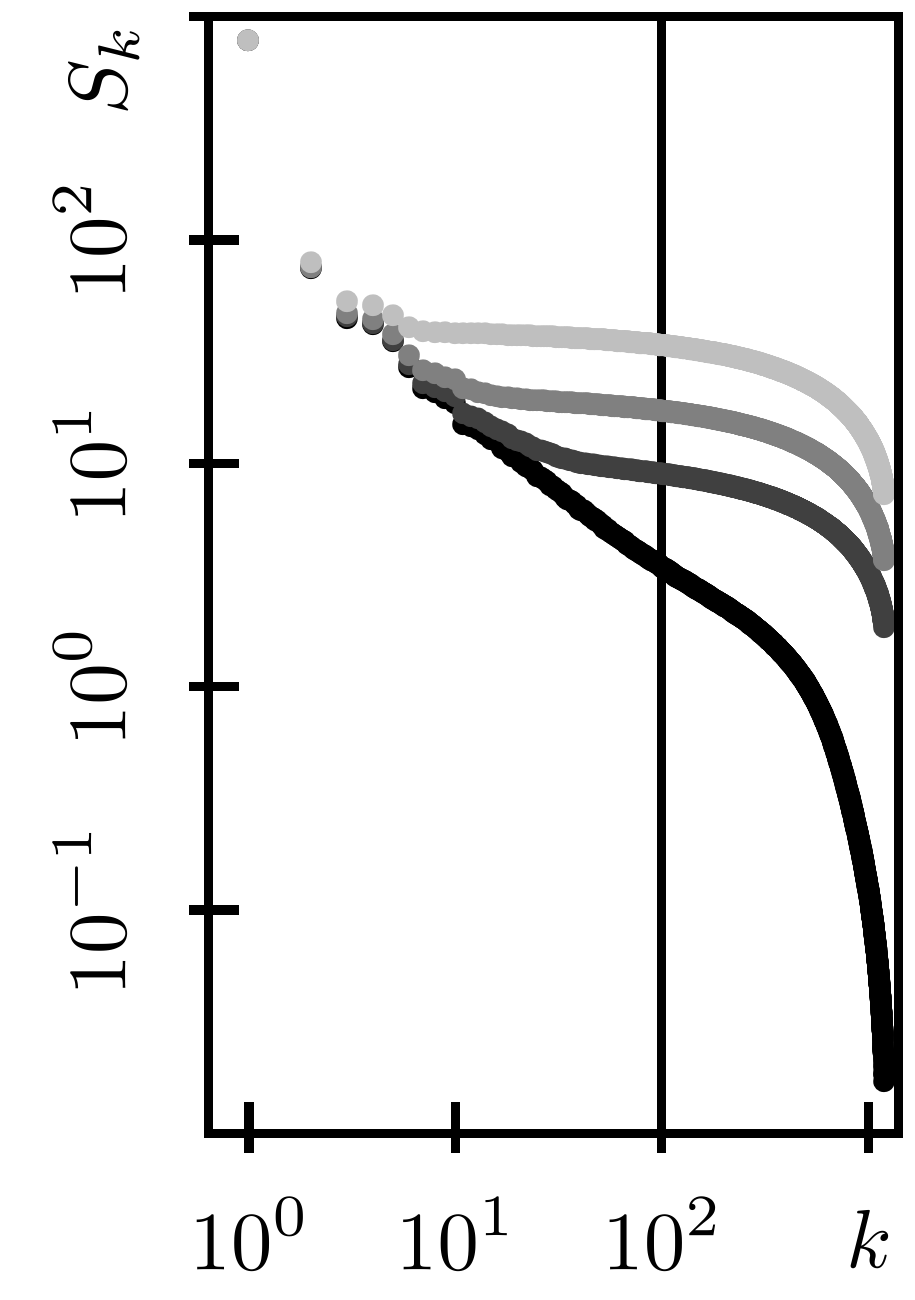
\includegraphics{figures/mandelbrot_svds.png}}
    \hfil
    \subfigure[]{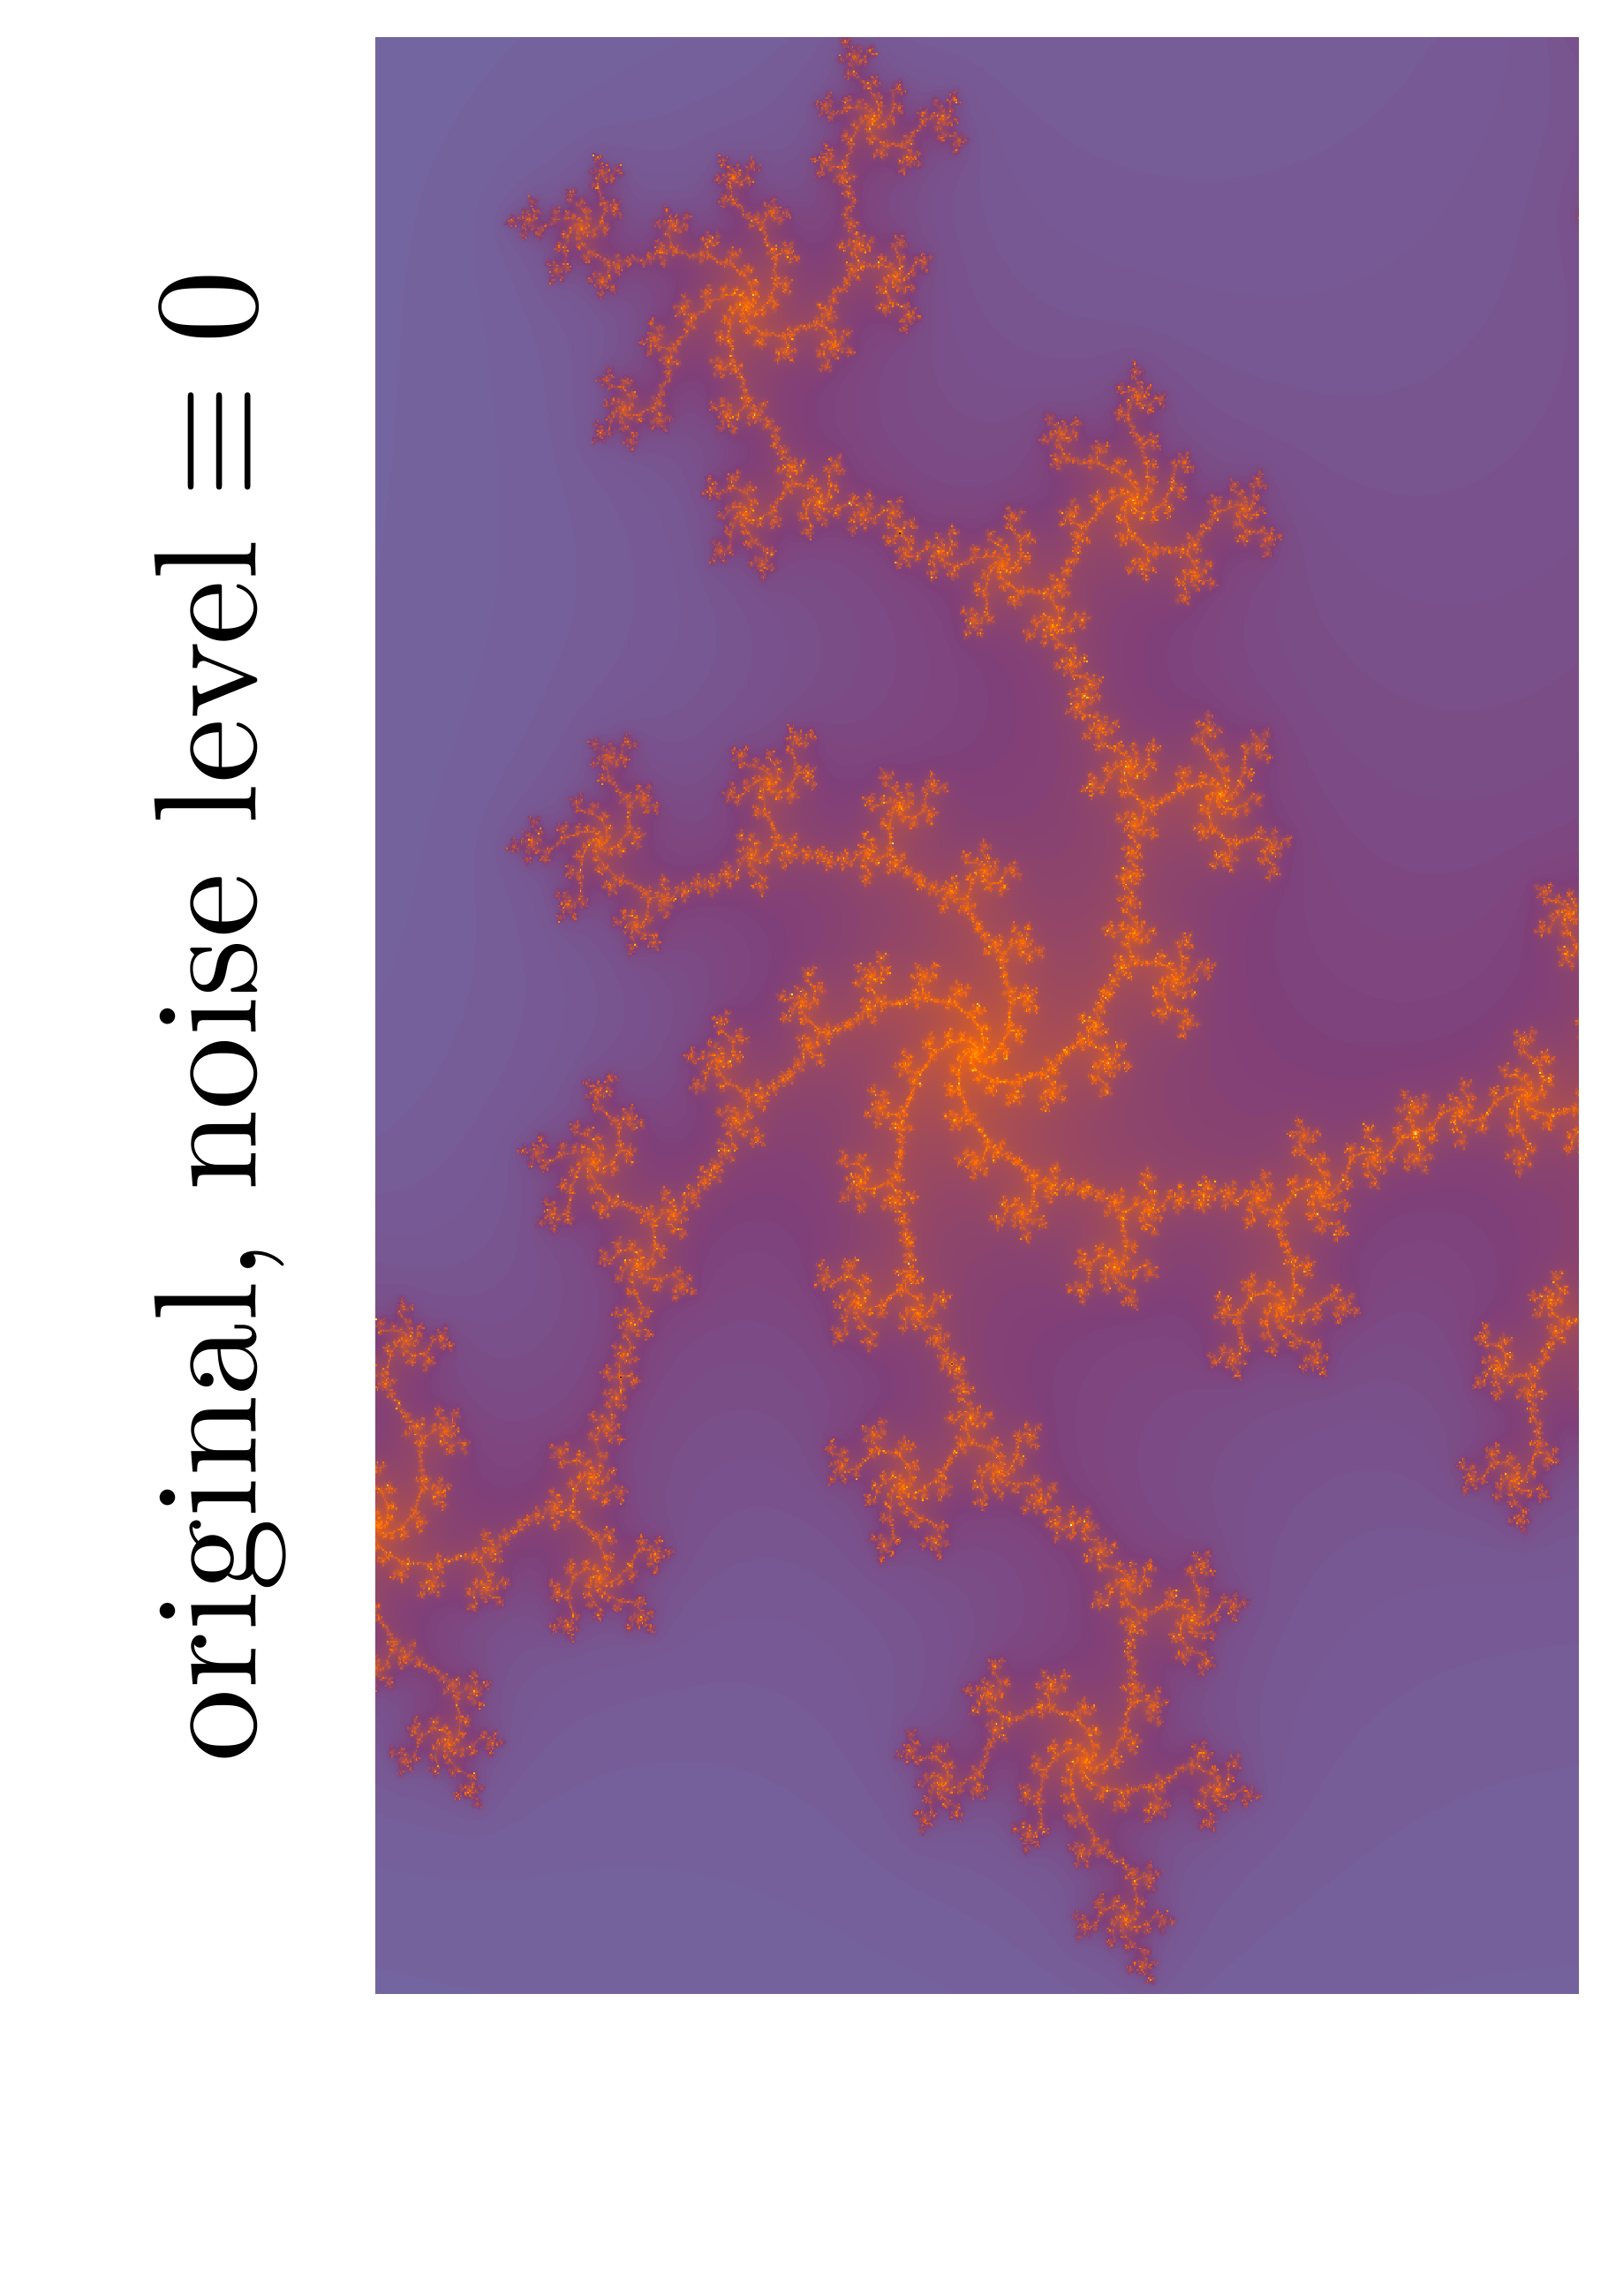
\includegraphics{figures/mandelbrot_noise_original1.png}}
    \hfil
    \subfigure[]{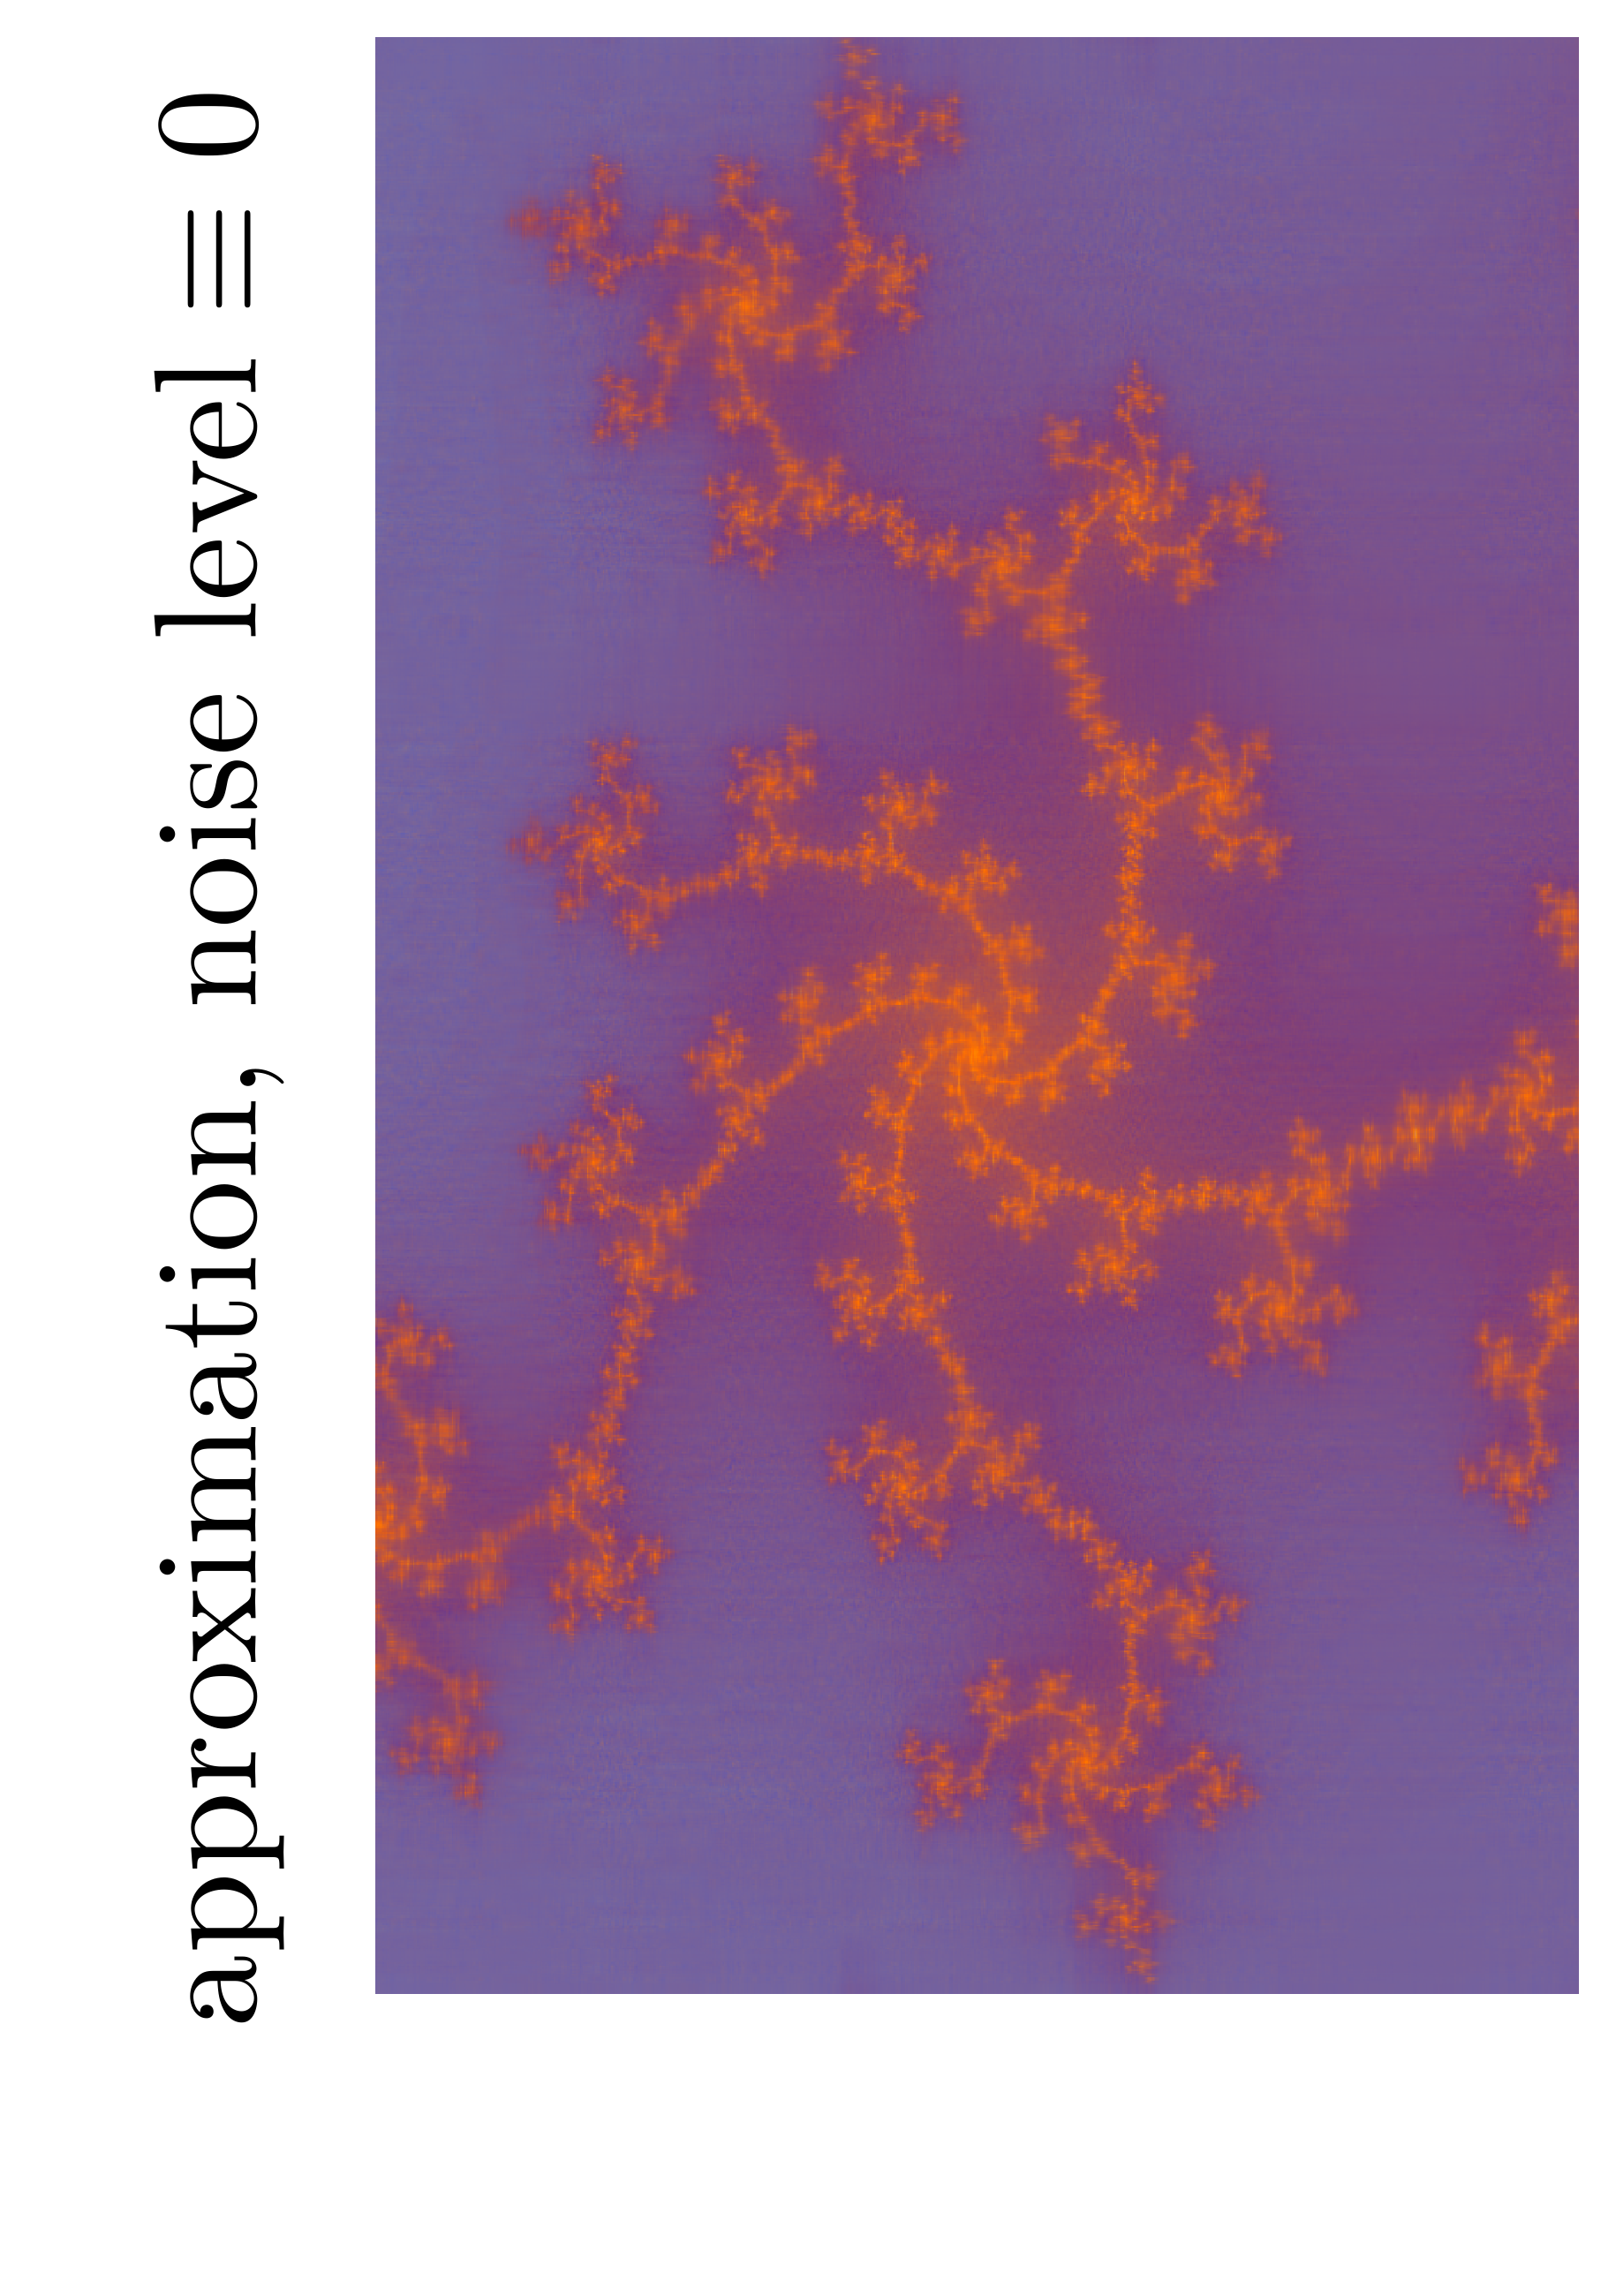
\includegraphics{figures/mandelbrot_noise_approx1.png}}
    \\
    \subfigure[]{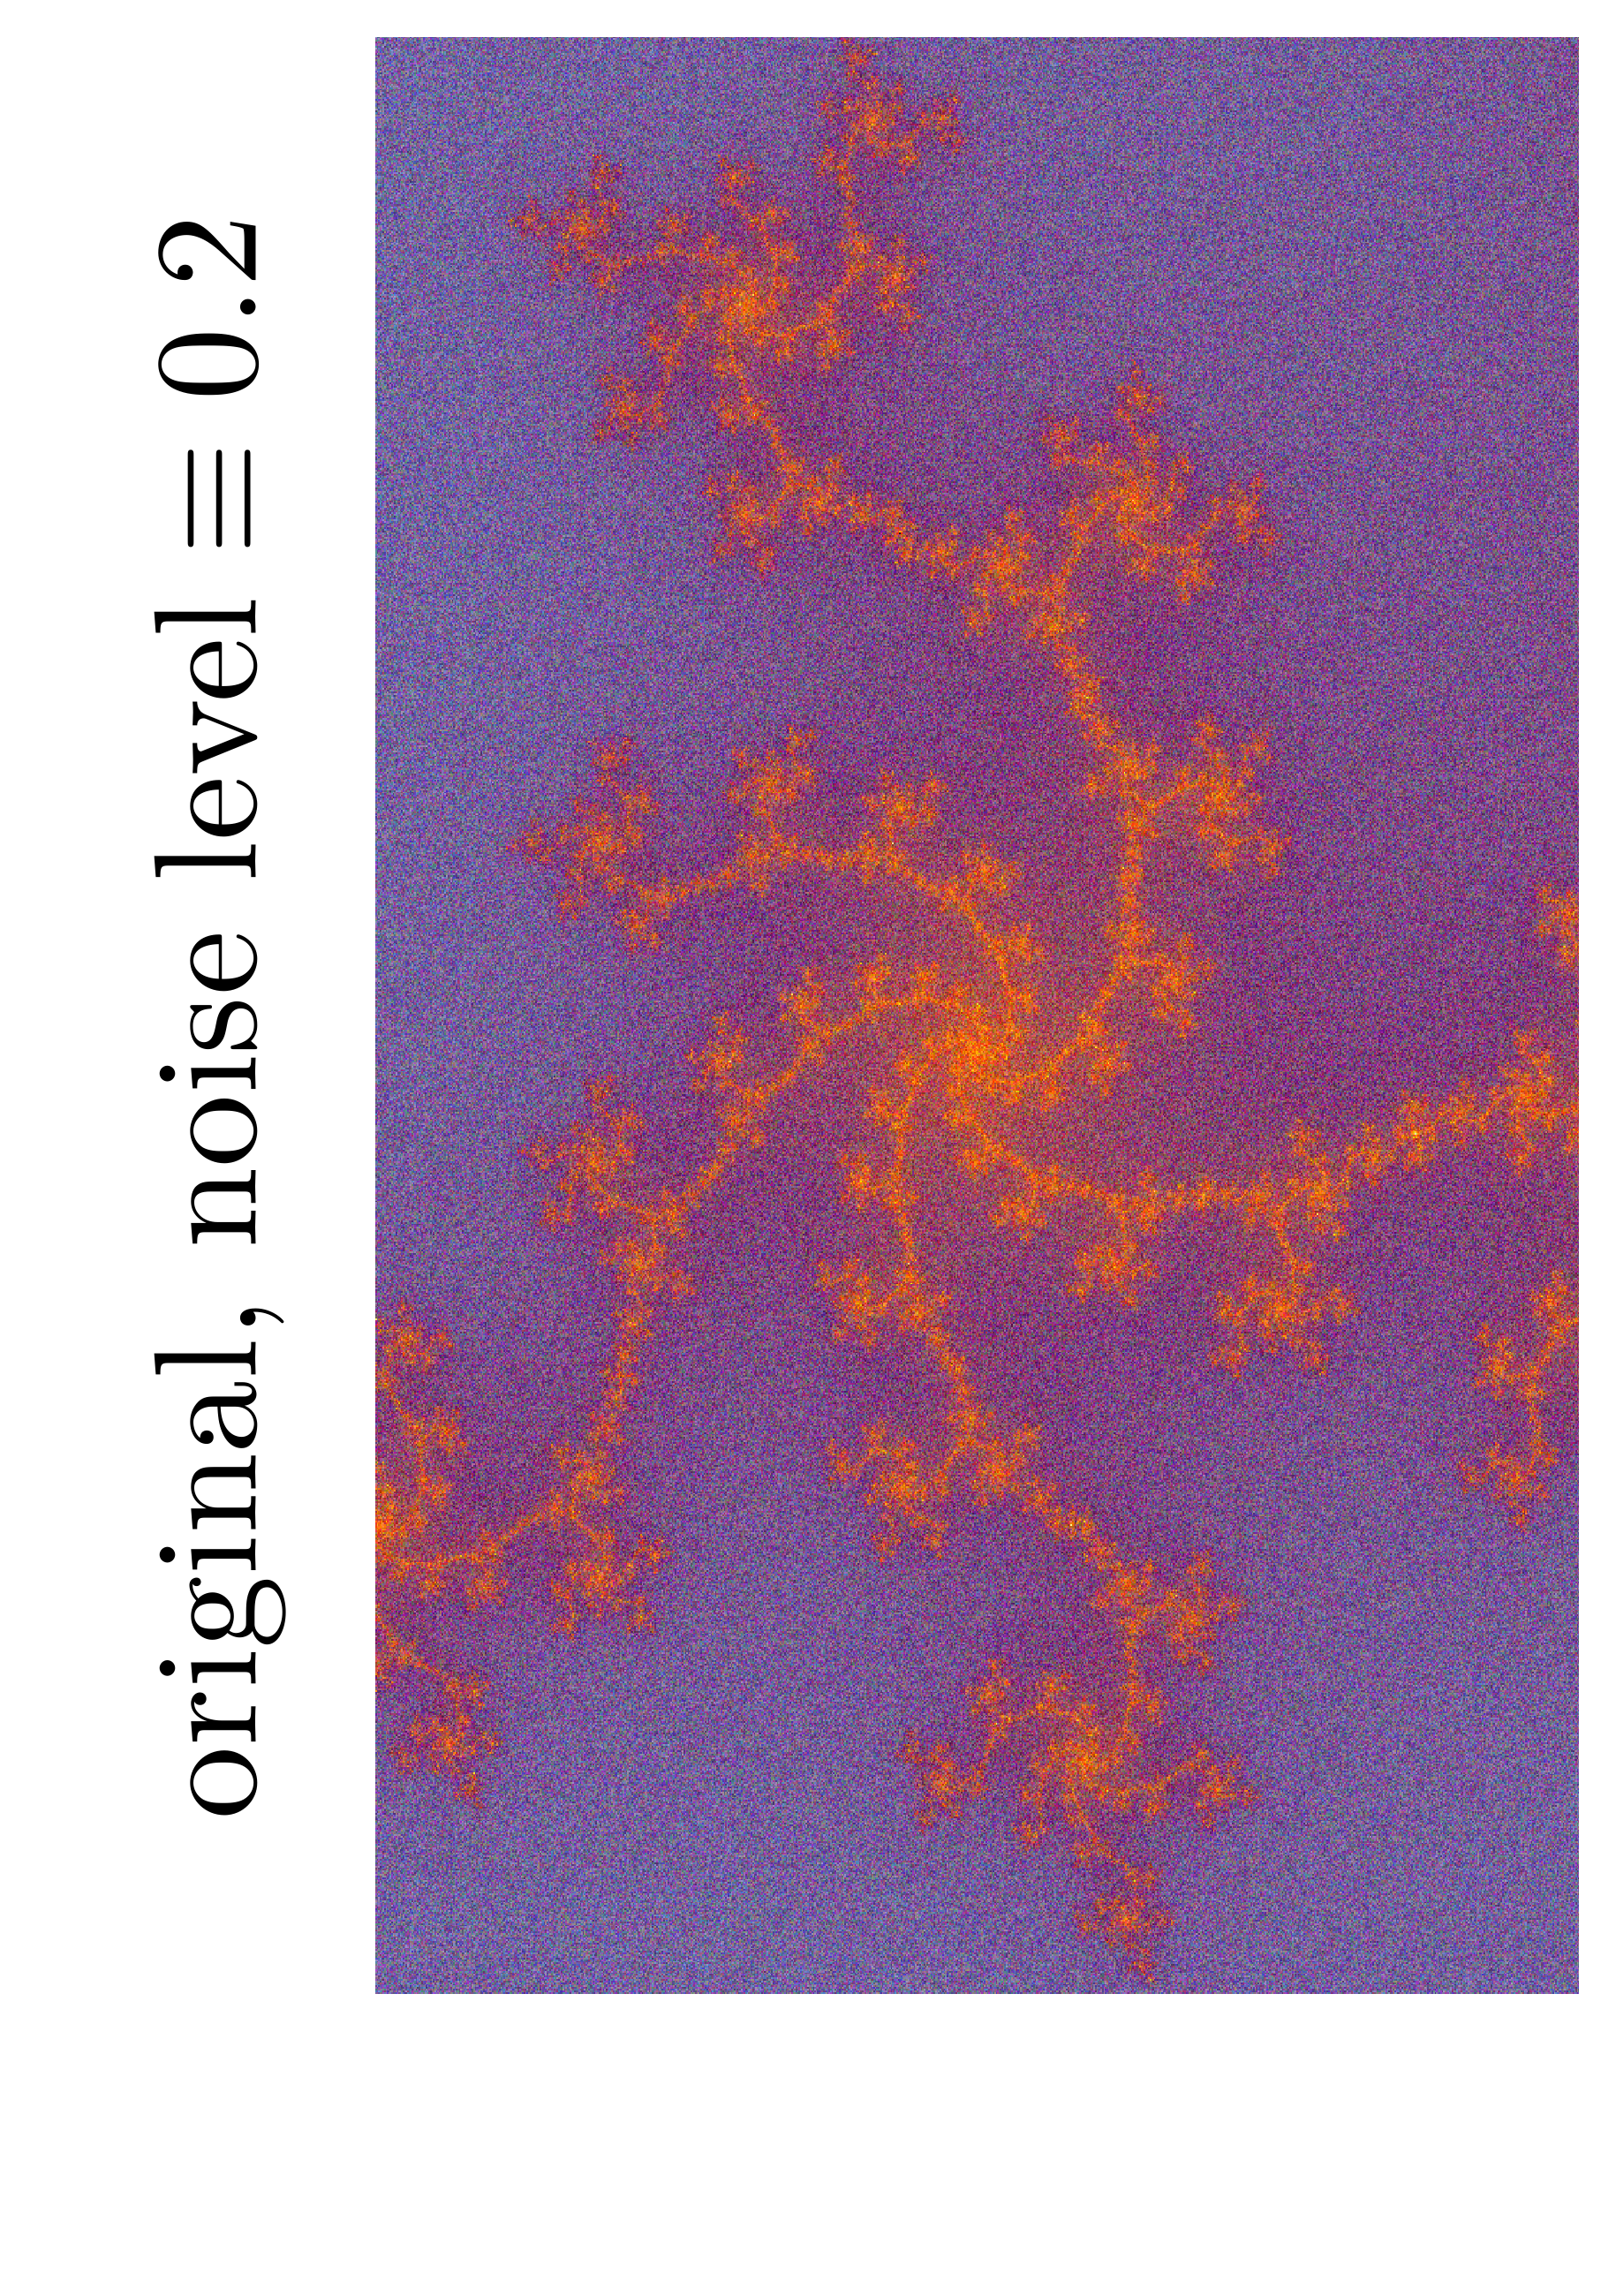
\includegraphics{figures/mandelbrot_noise_original4.png}}
    \hfil
    \subfigure[]{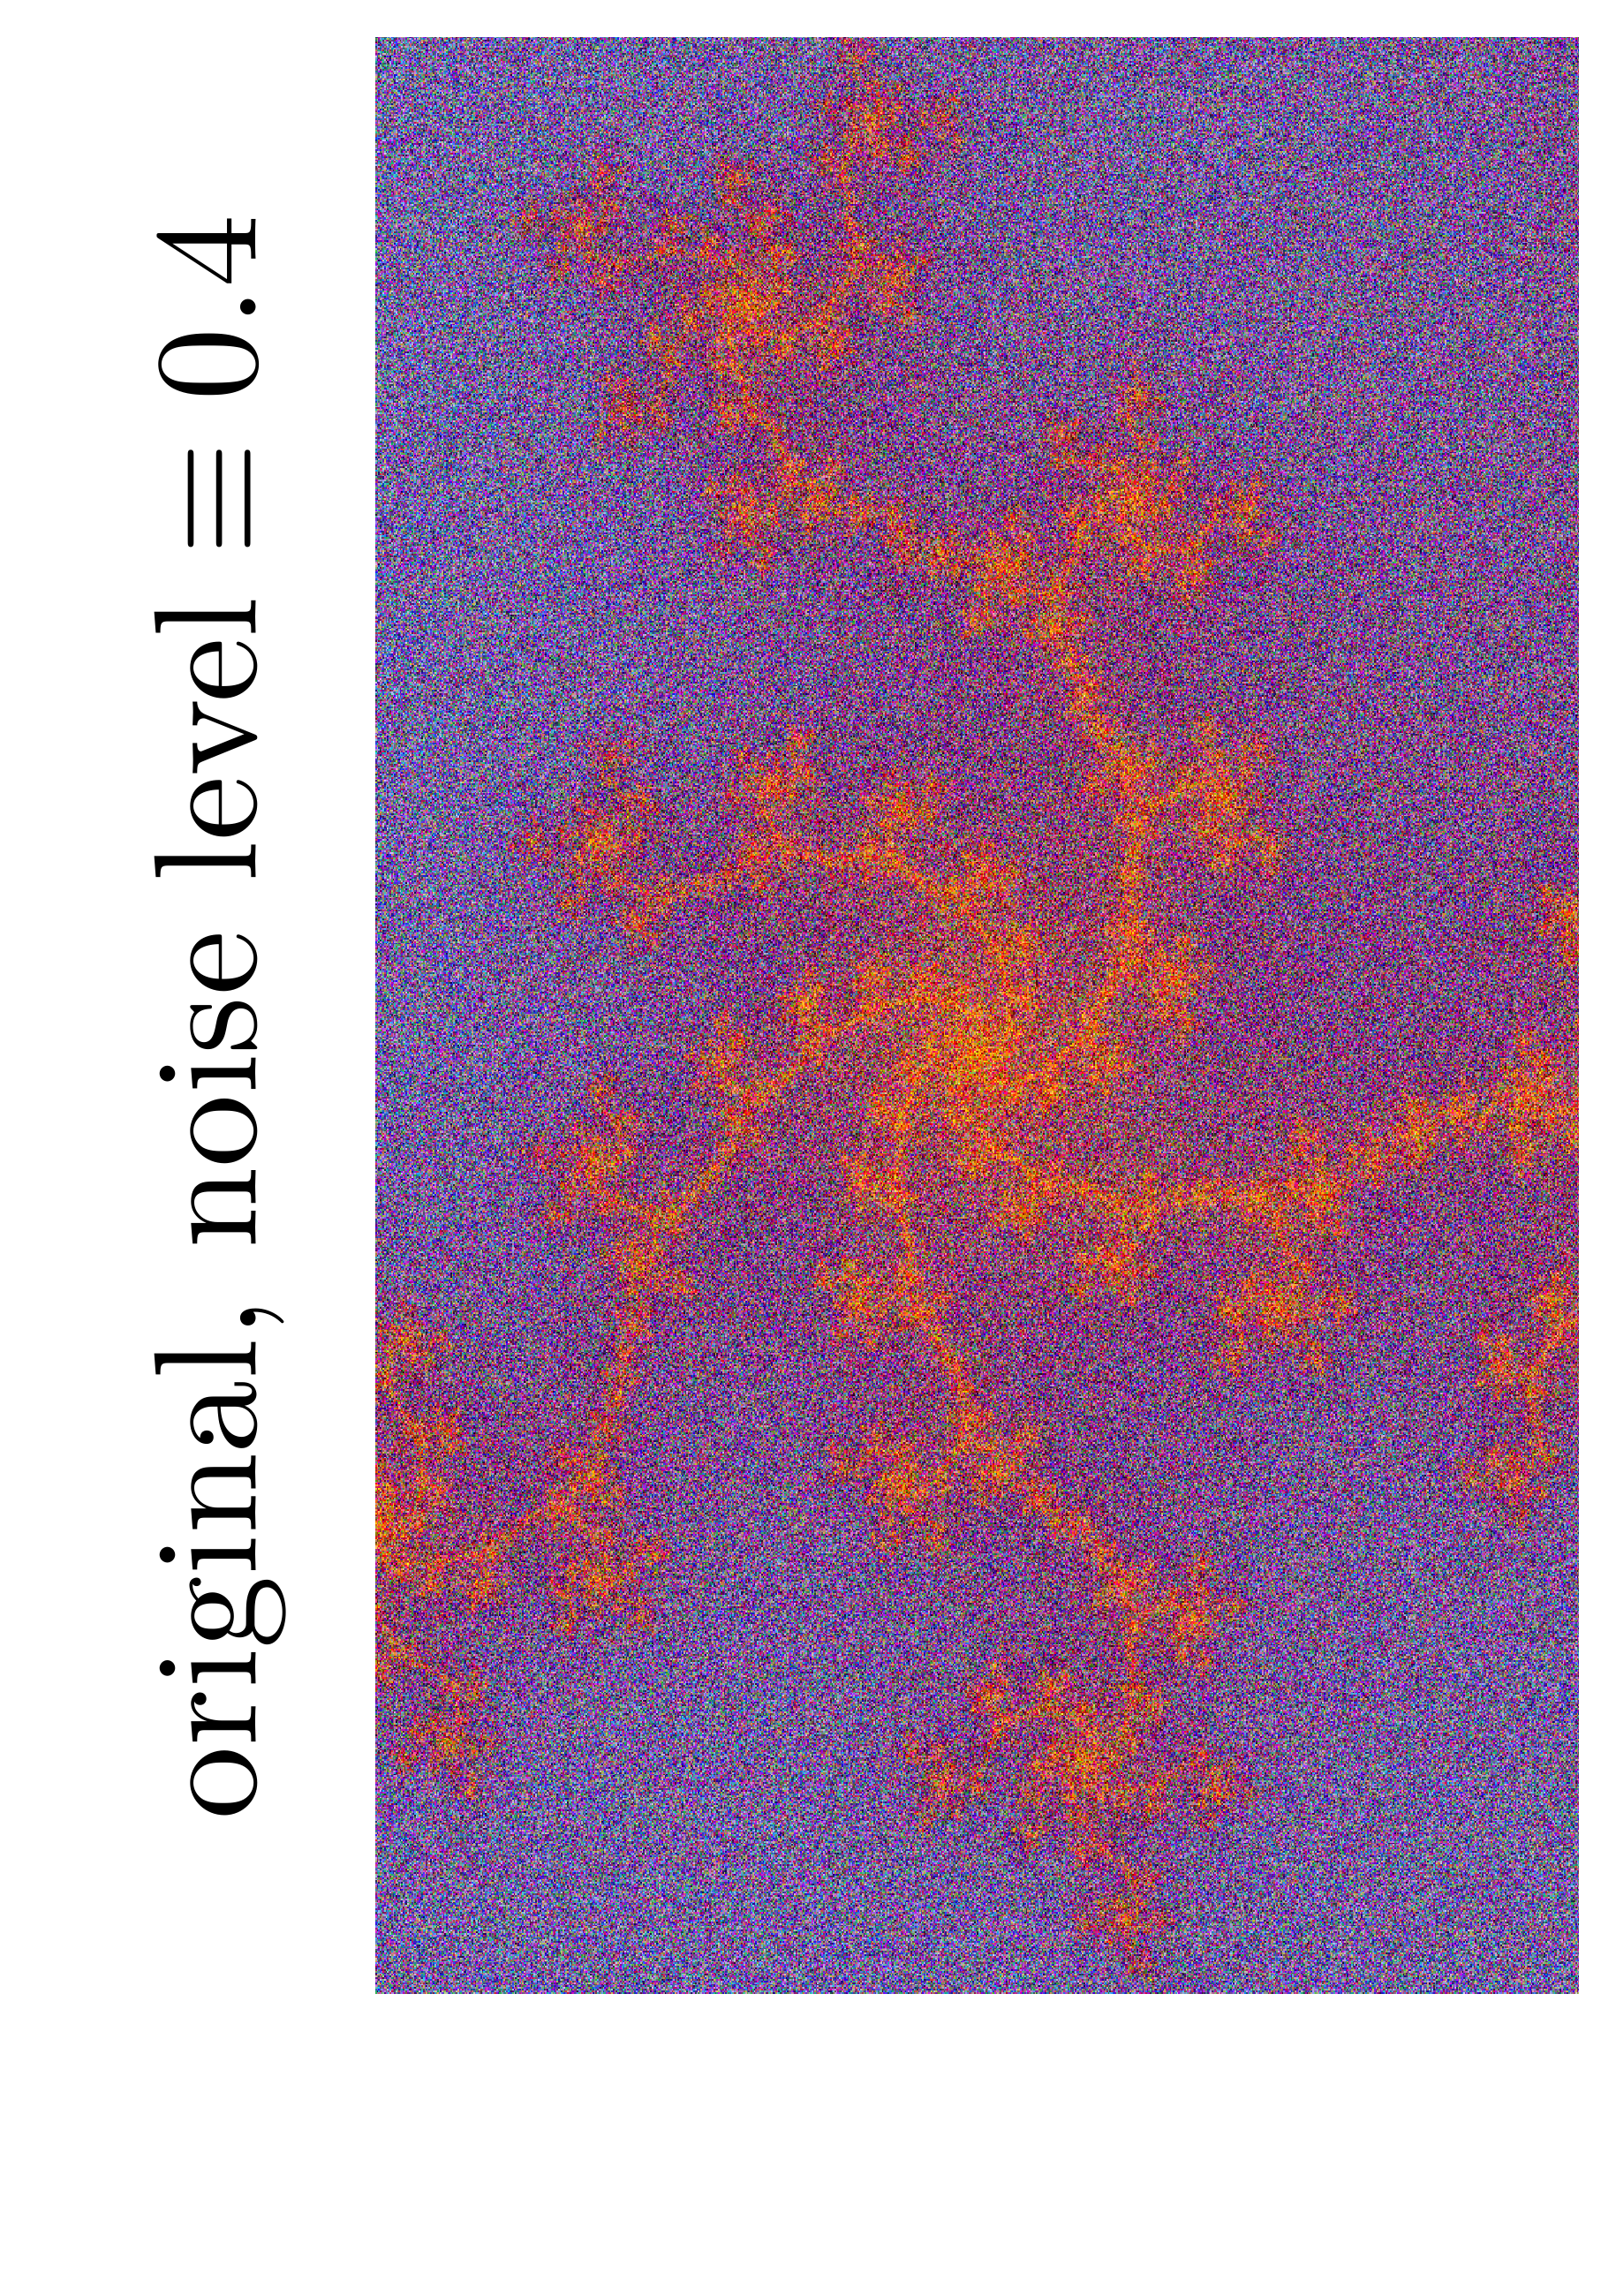
\includegraphics{figures/mandelbrot_noise_original5.png}}
    \hfil
    \subfigure[]{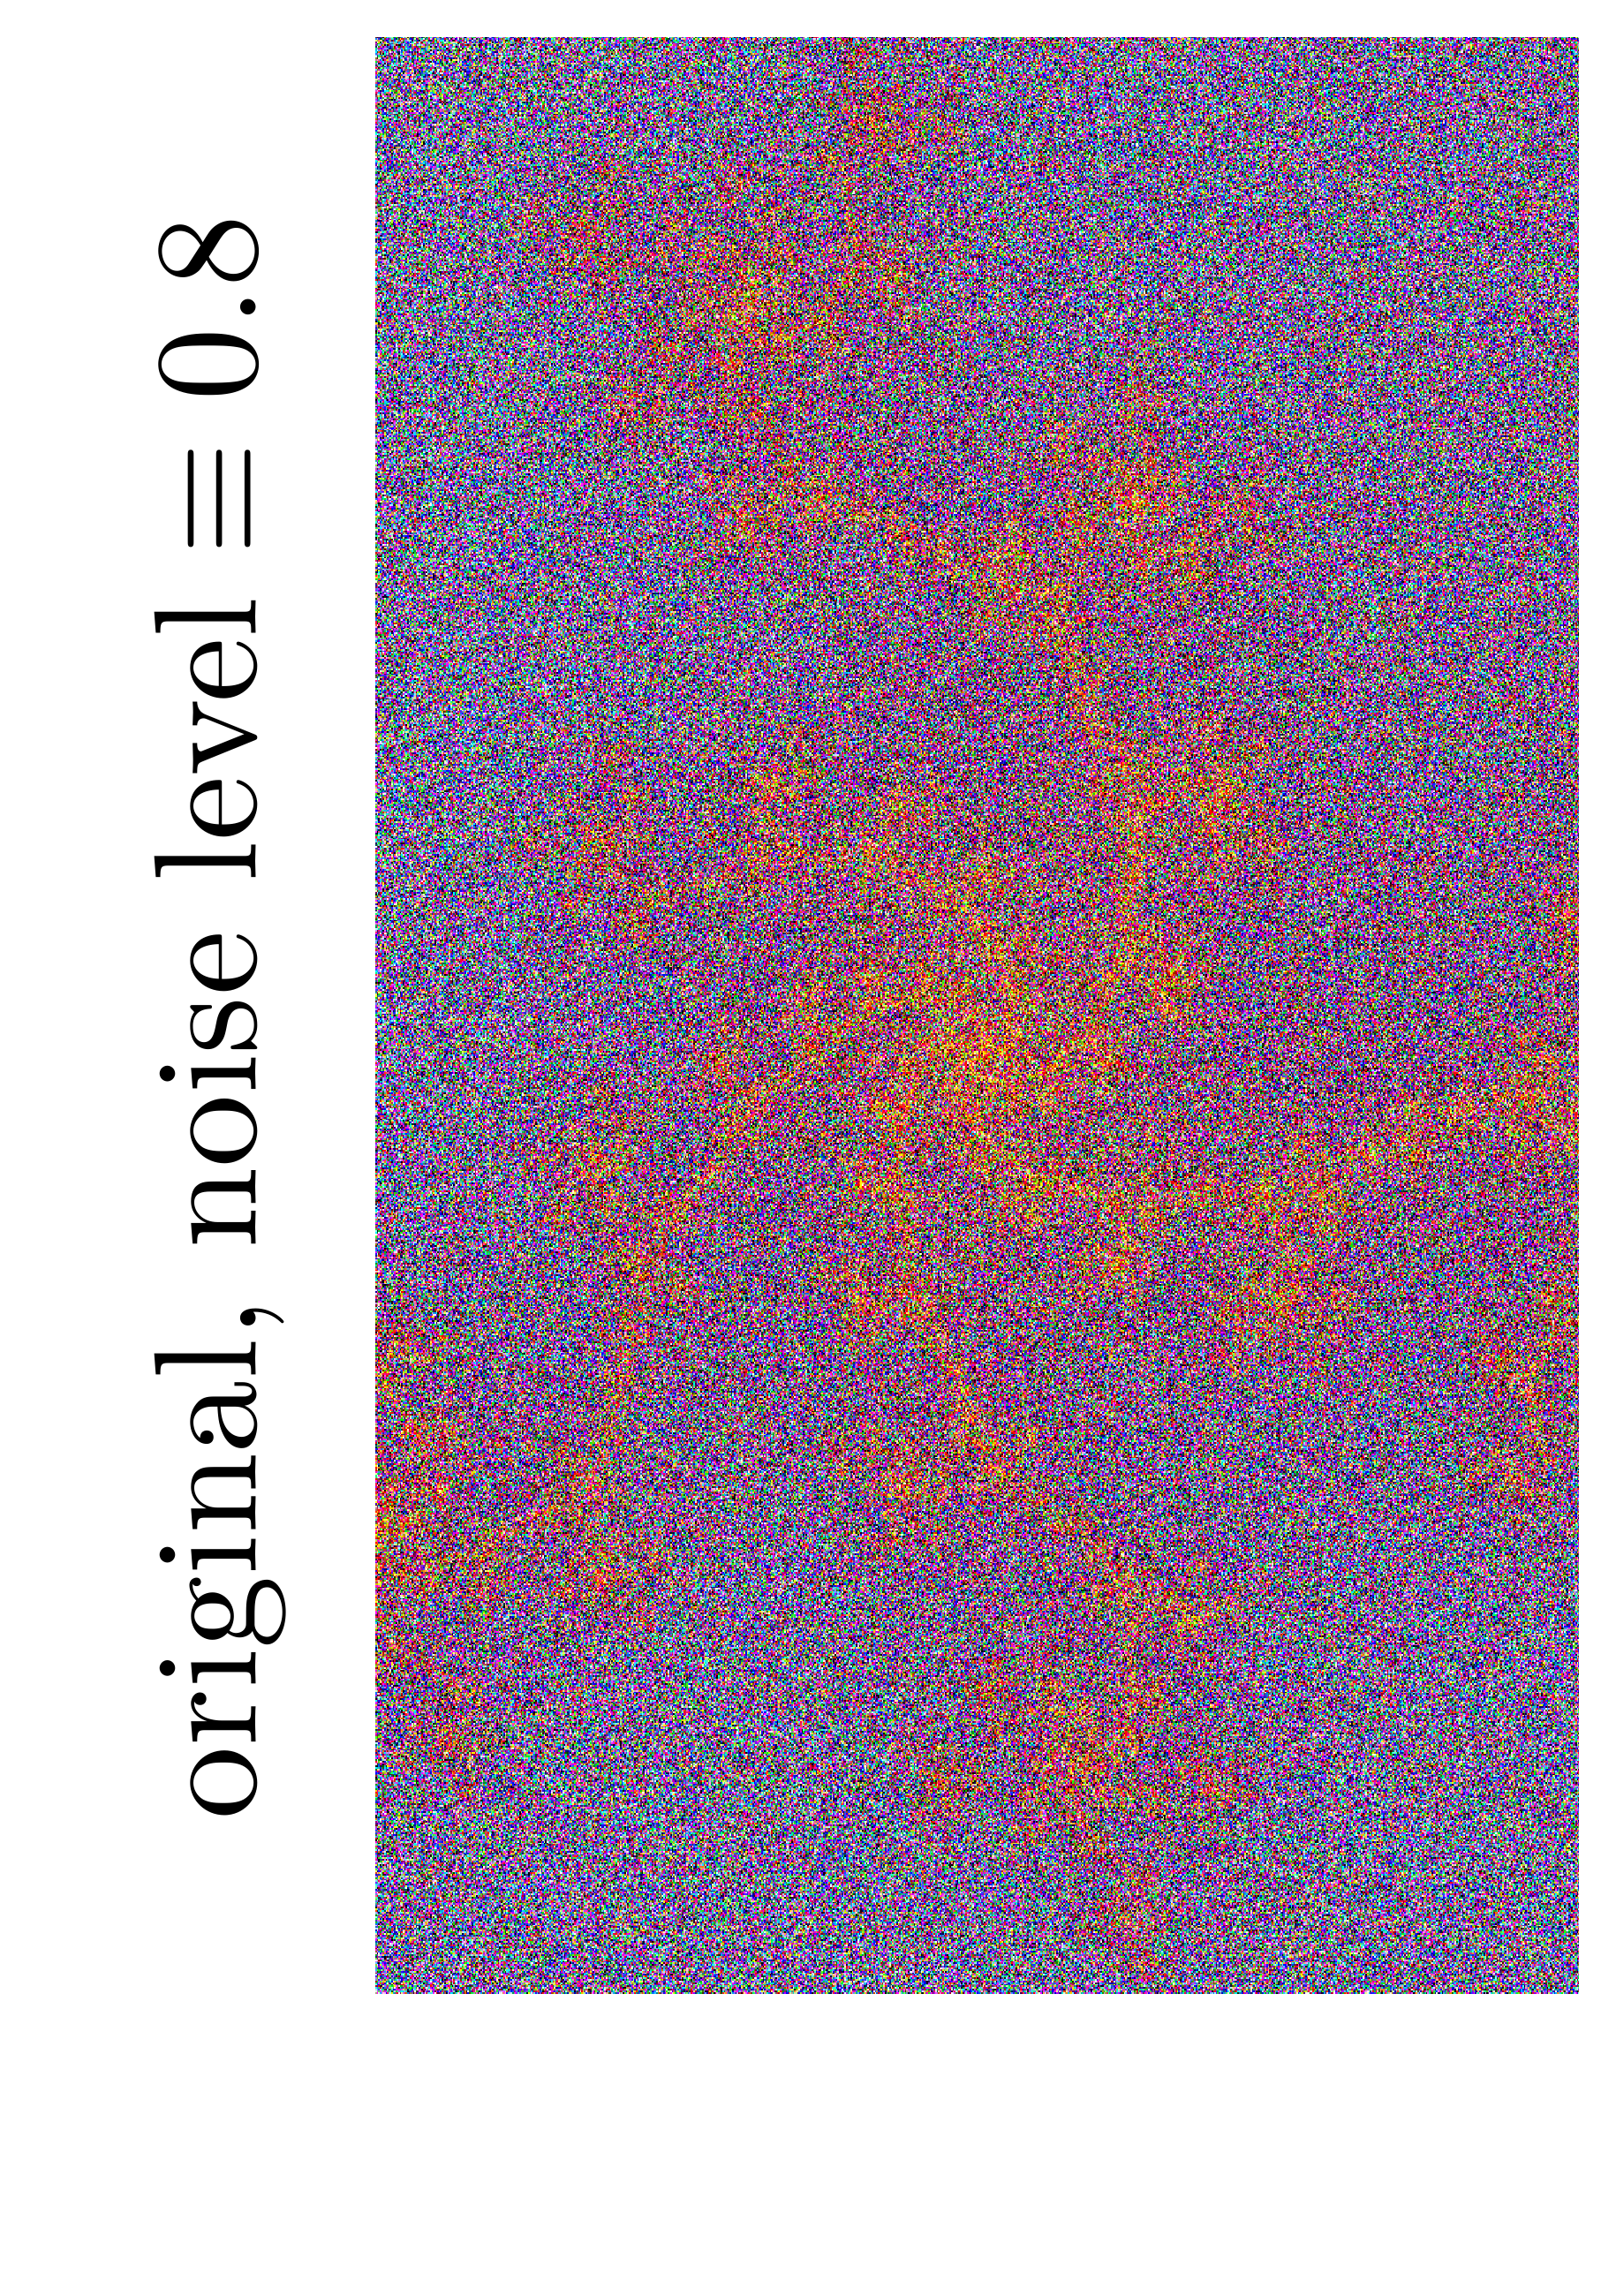
\includegraphics{figures/mandelbrot_noise_original6.png}}
    \\
    \subfigure[]{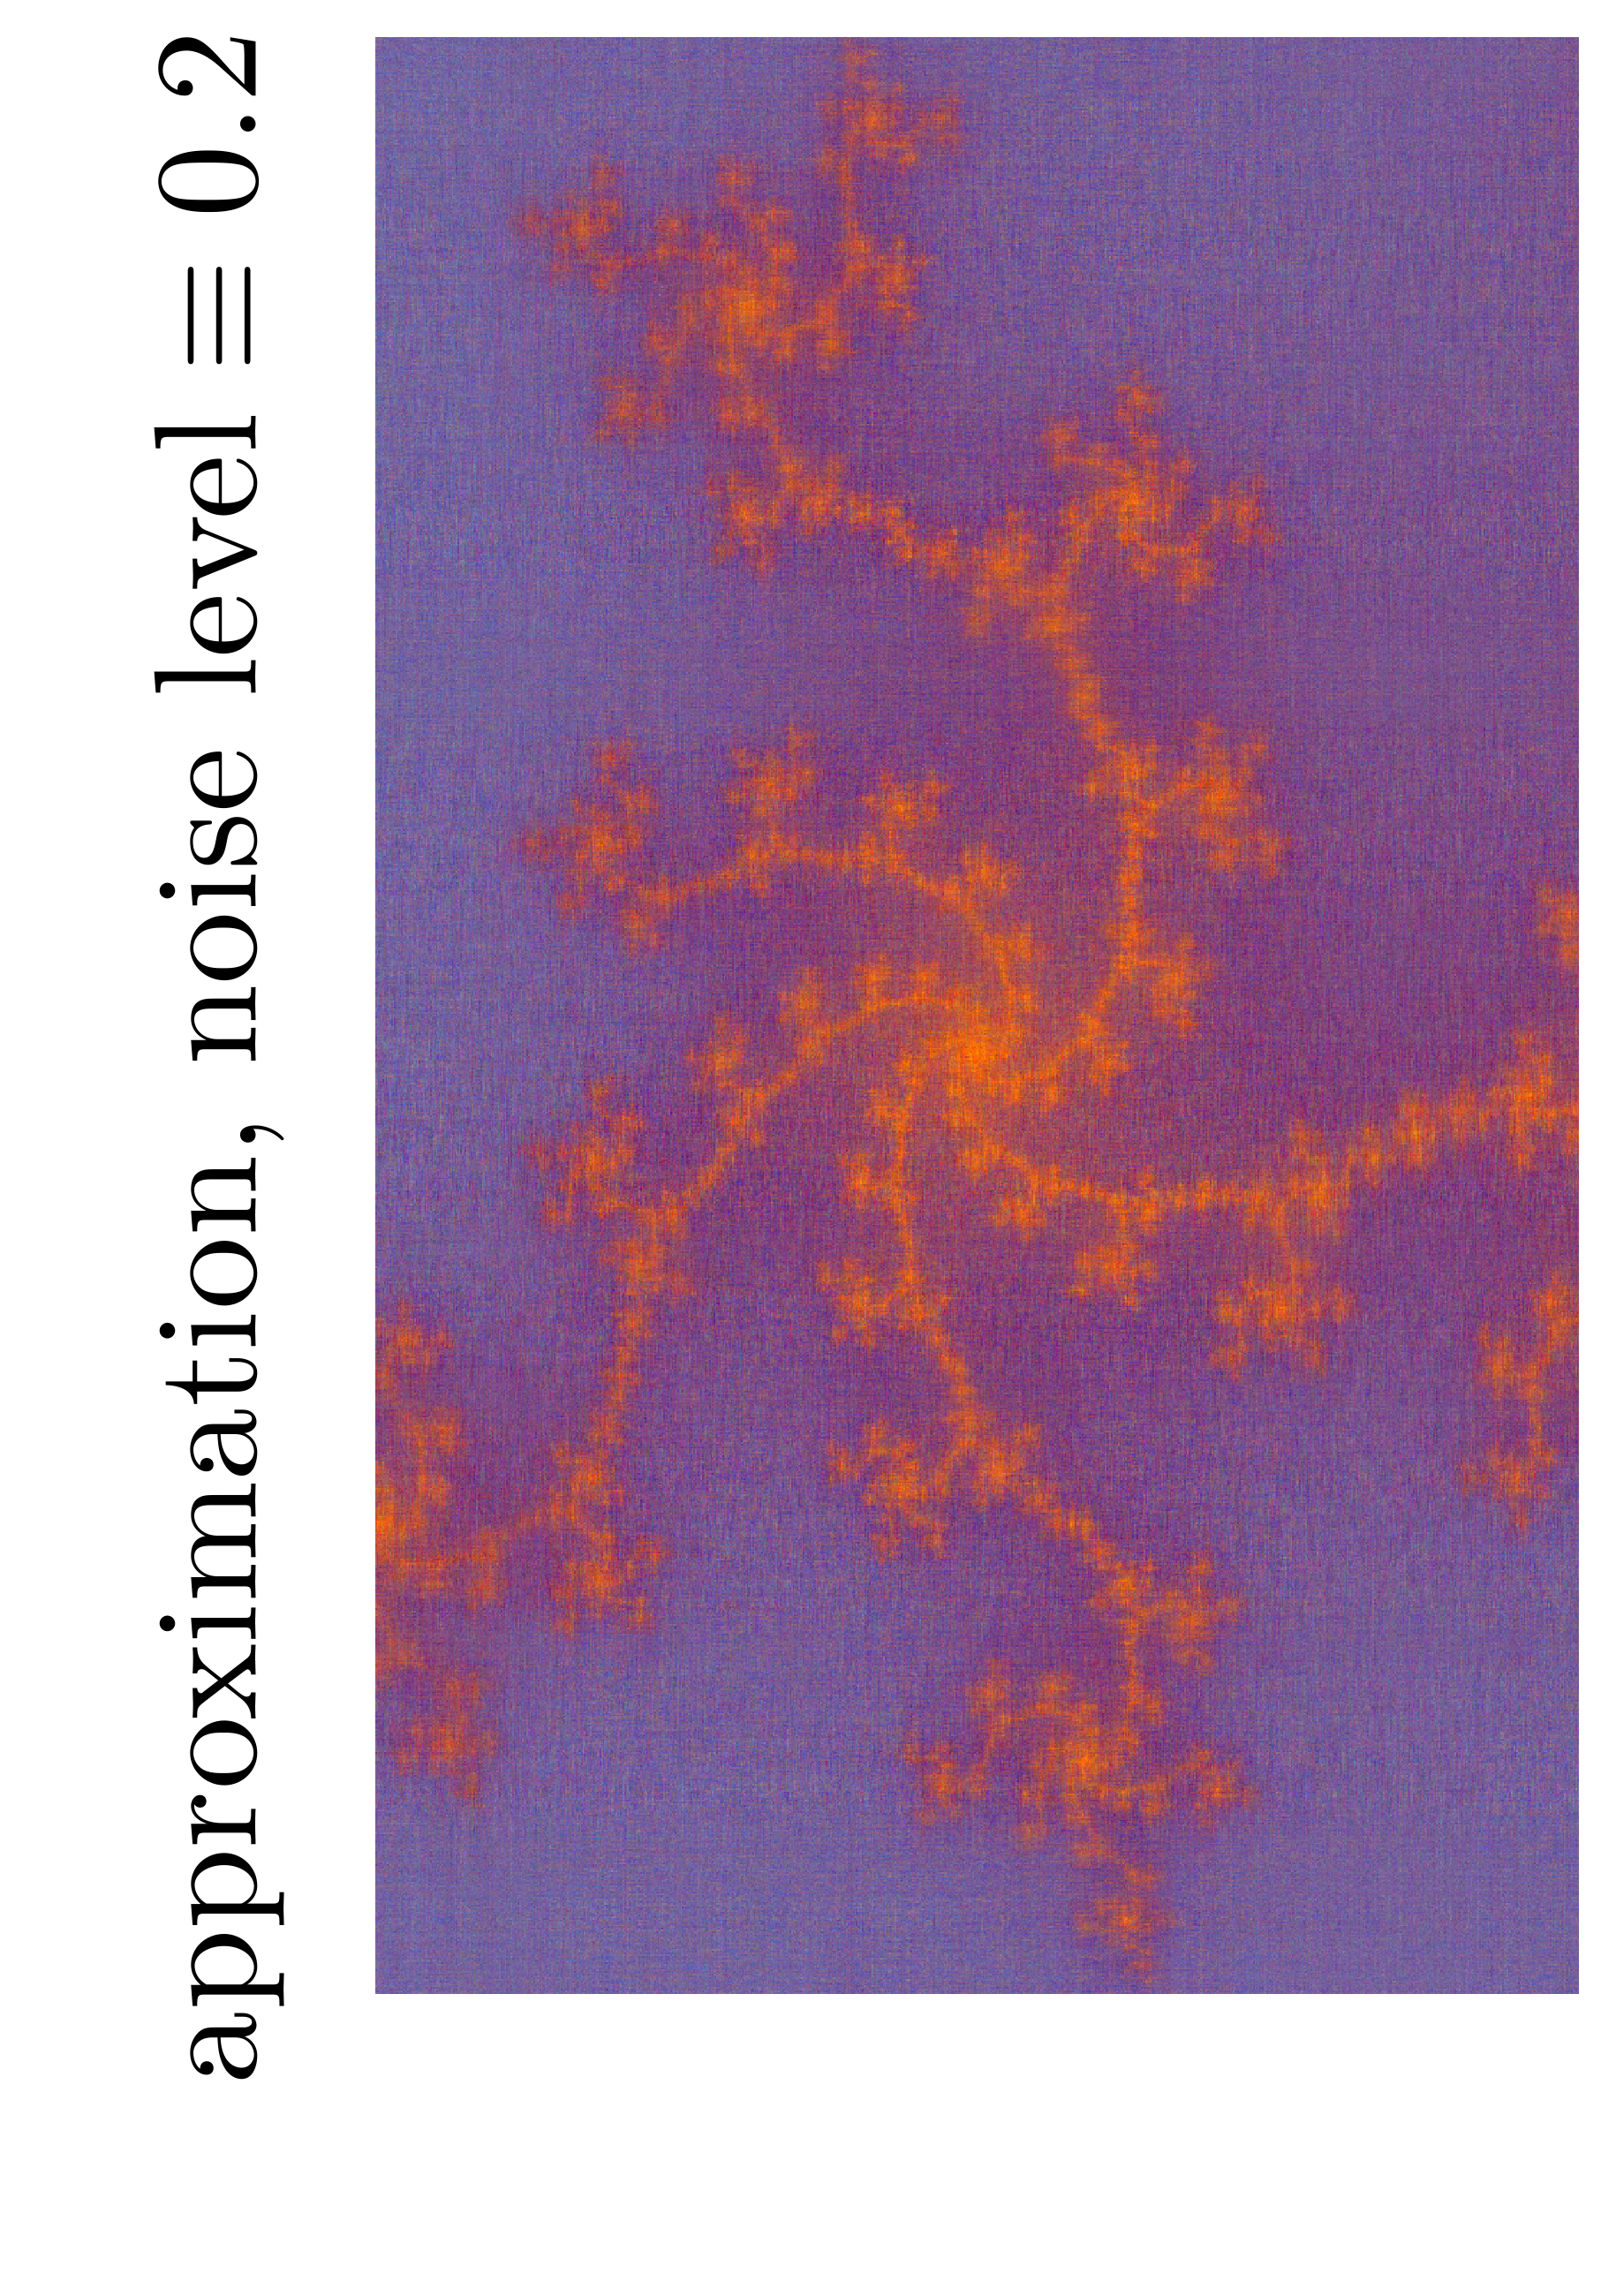
\includegraphics{figures/mandelbrot_noise_approx4.png}}
    \hfil
    \subfigure[]{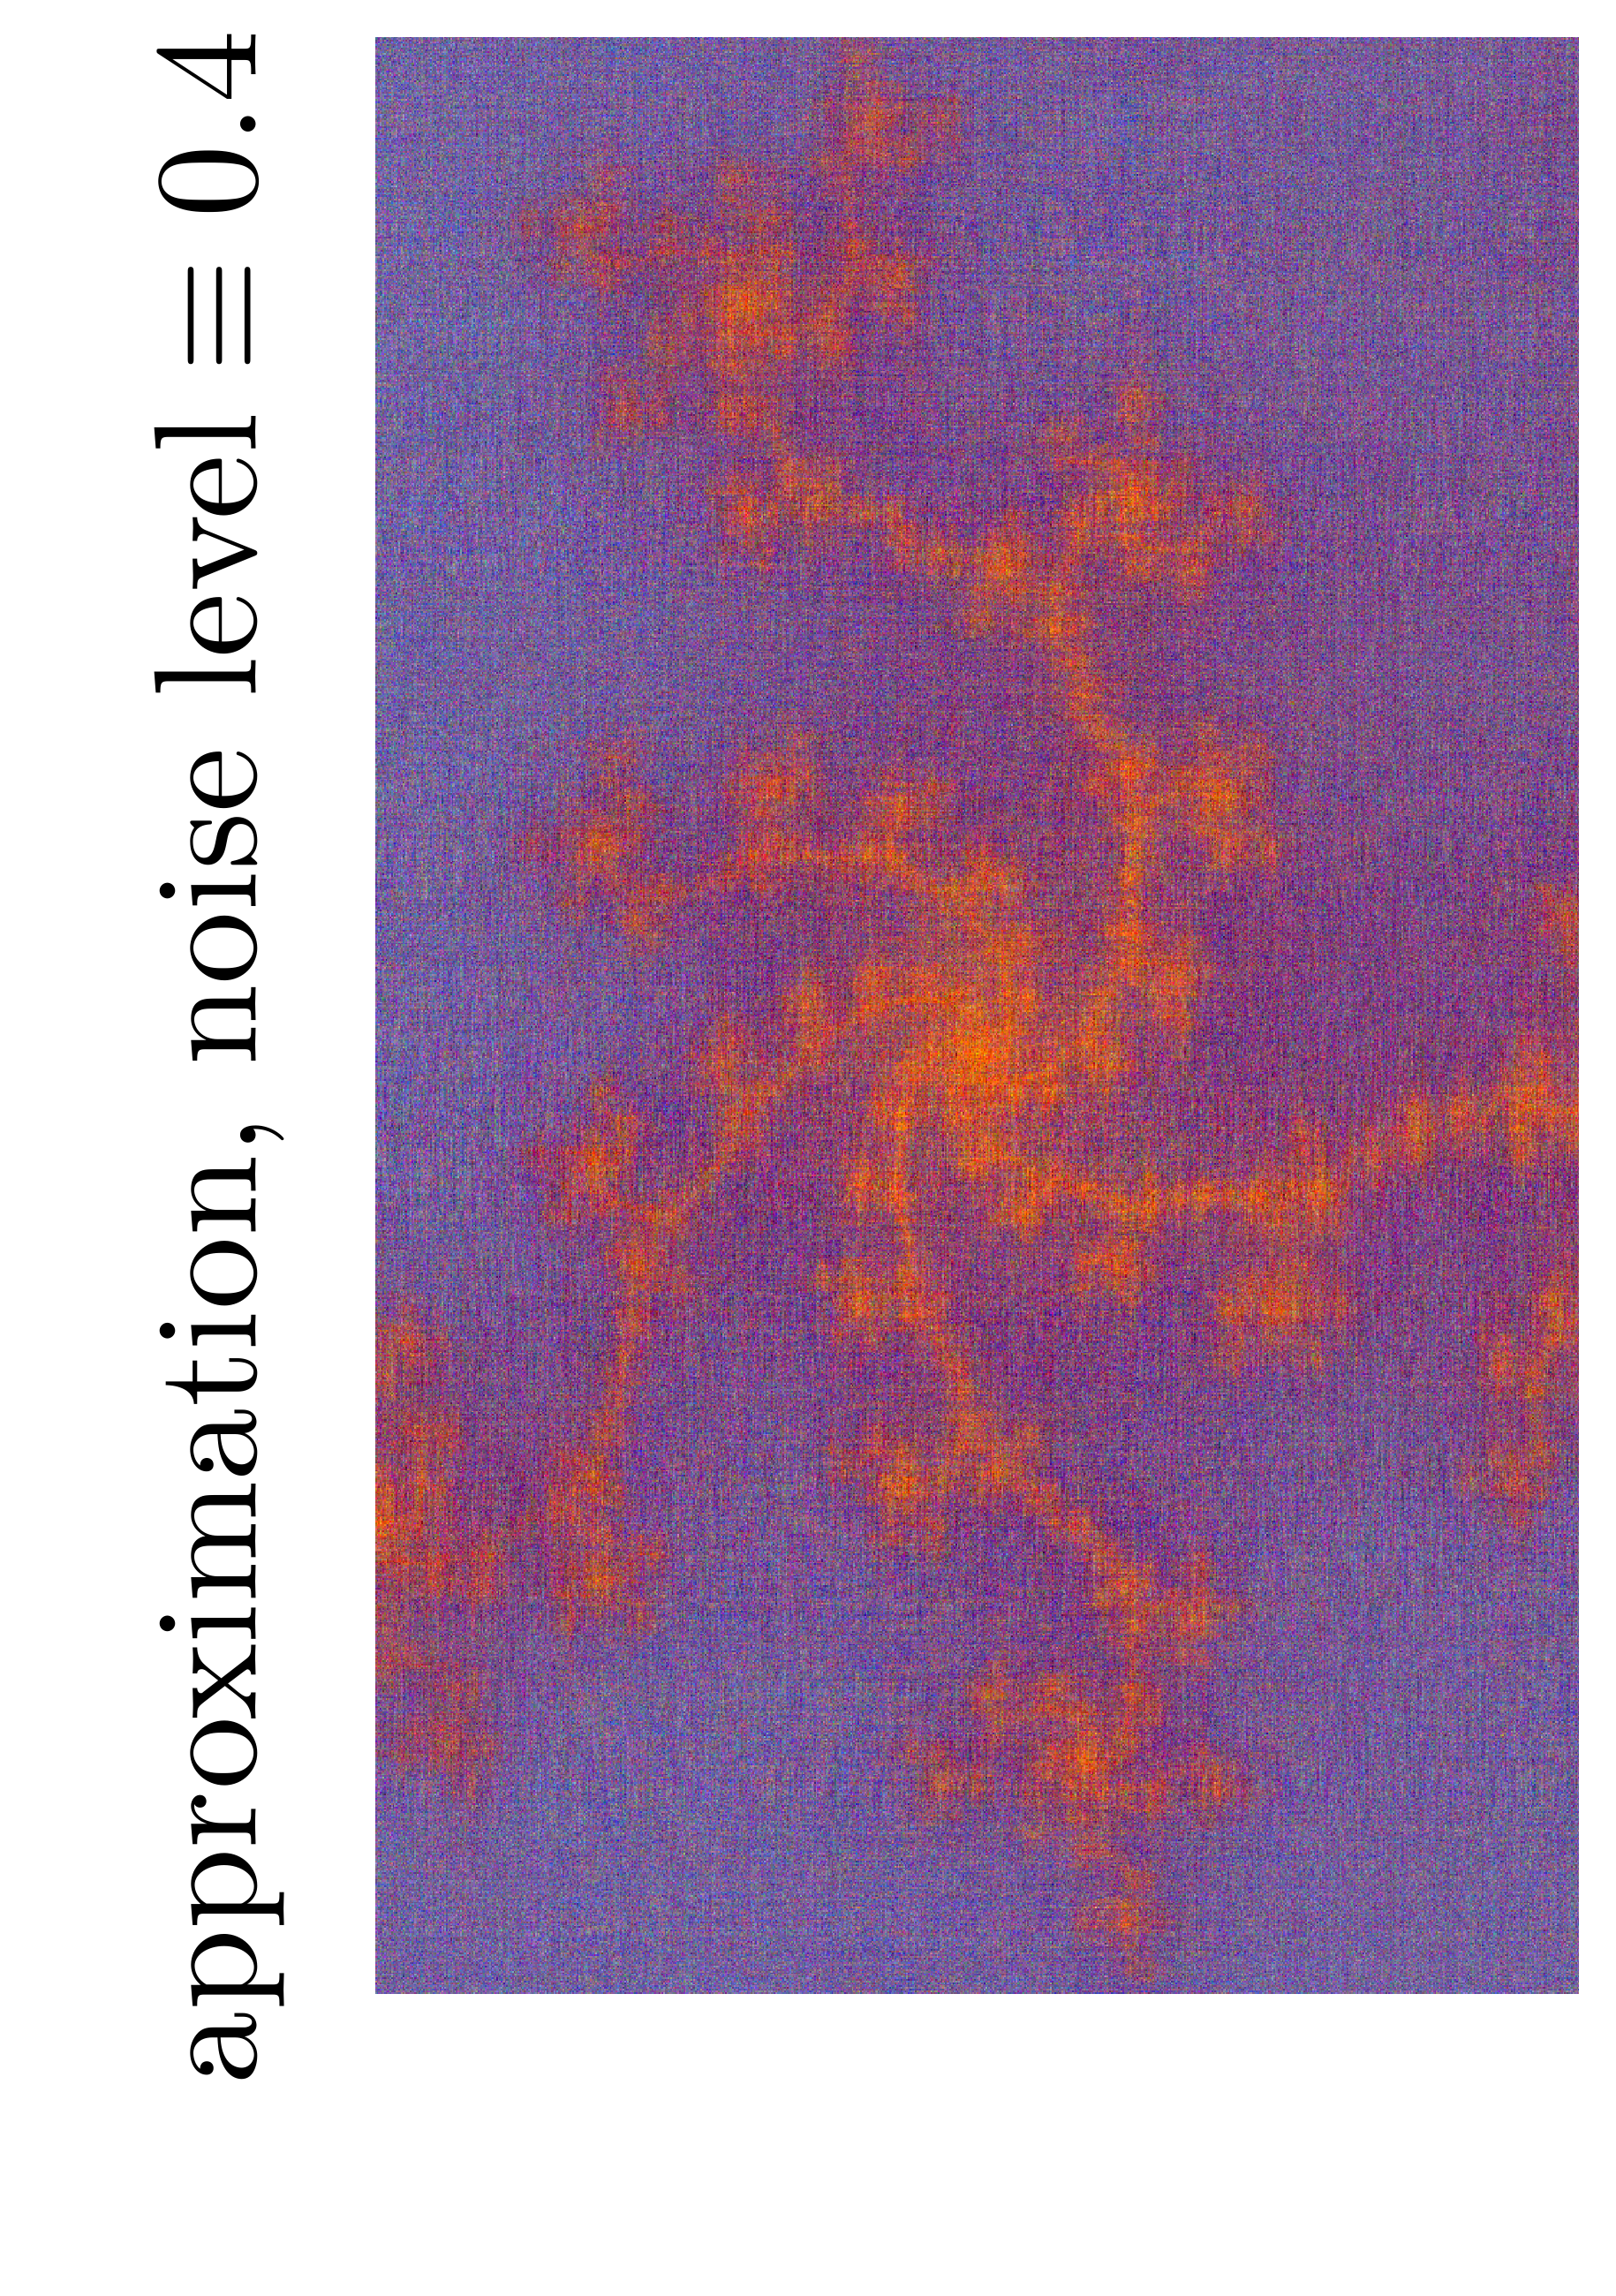
\includegraphics{figures/mandelbrot_noise_approx5.png}}
    \hfil
    \subfigure[]{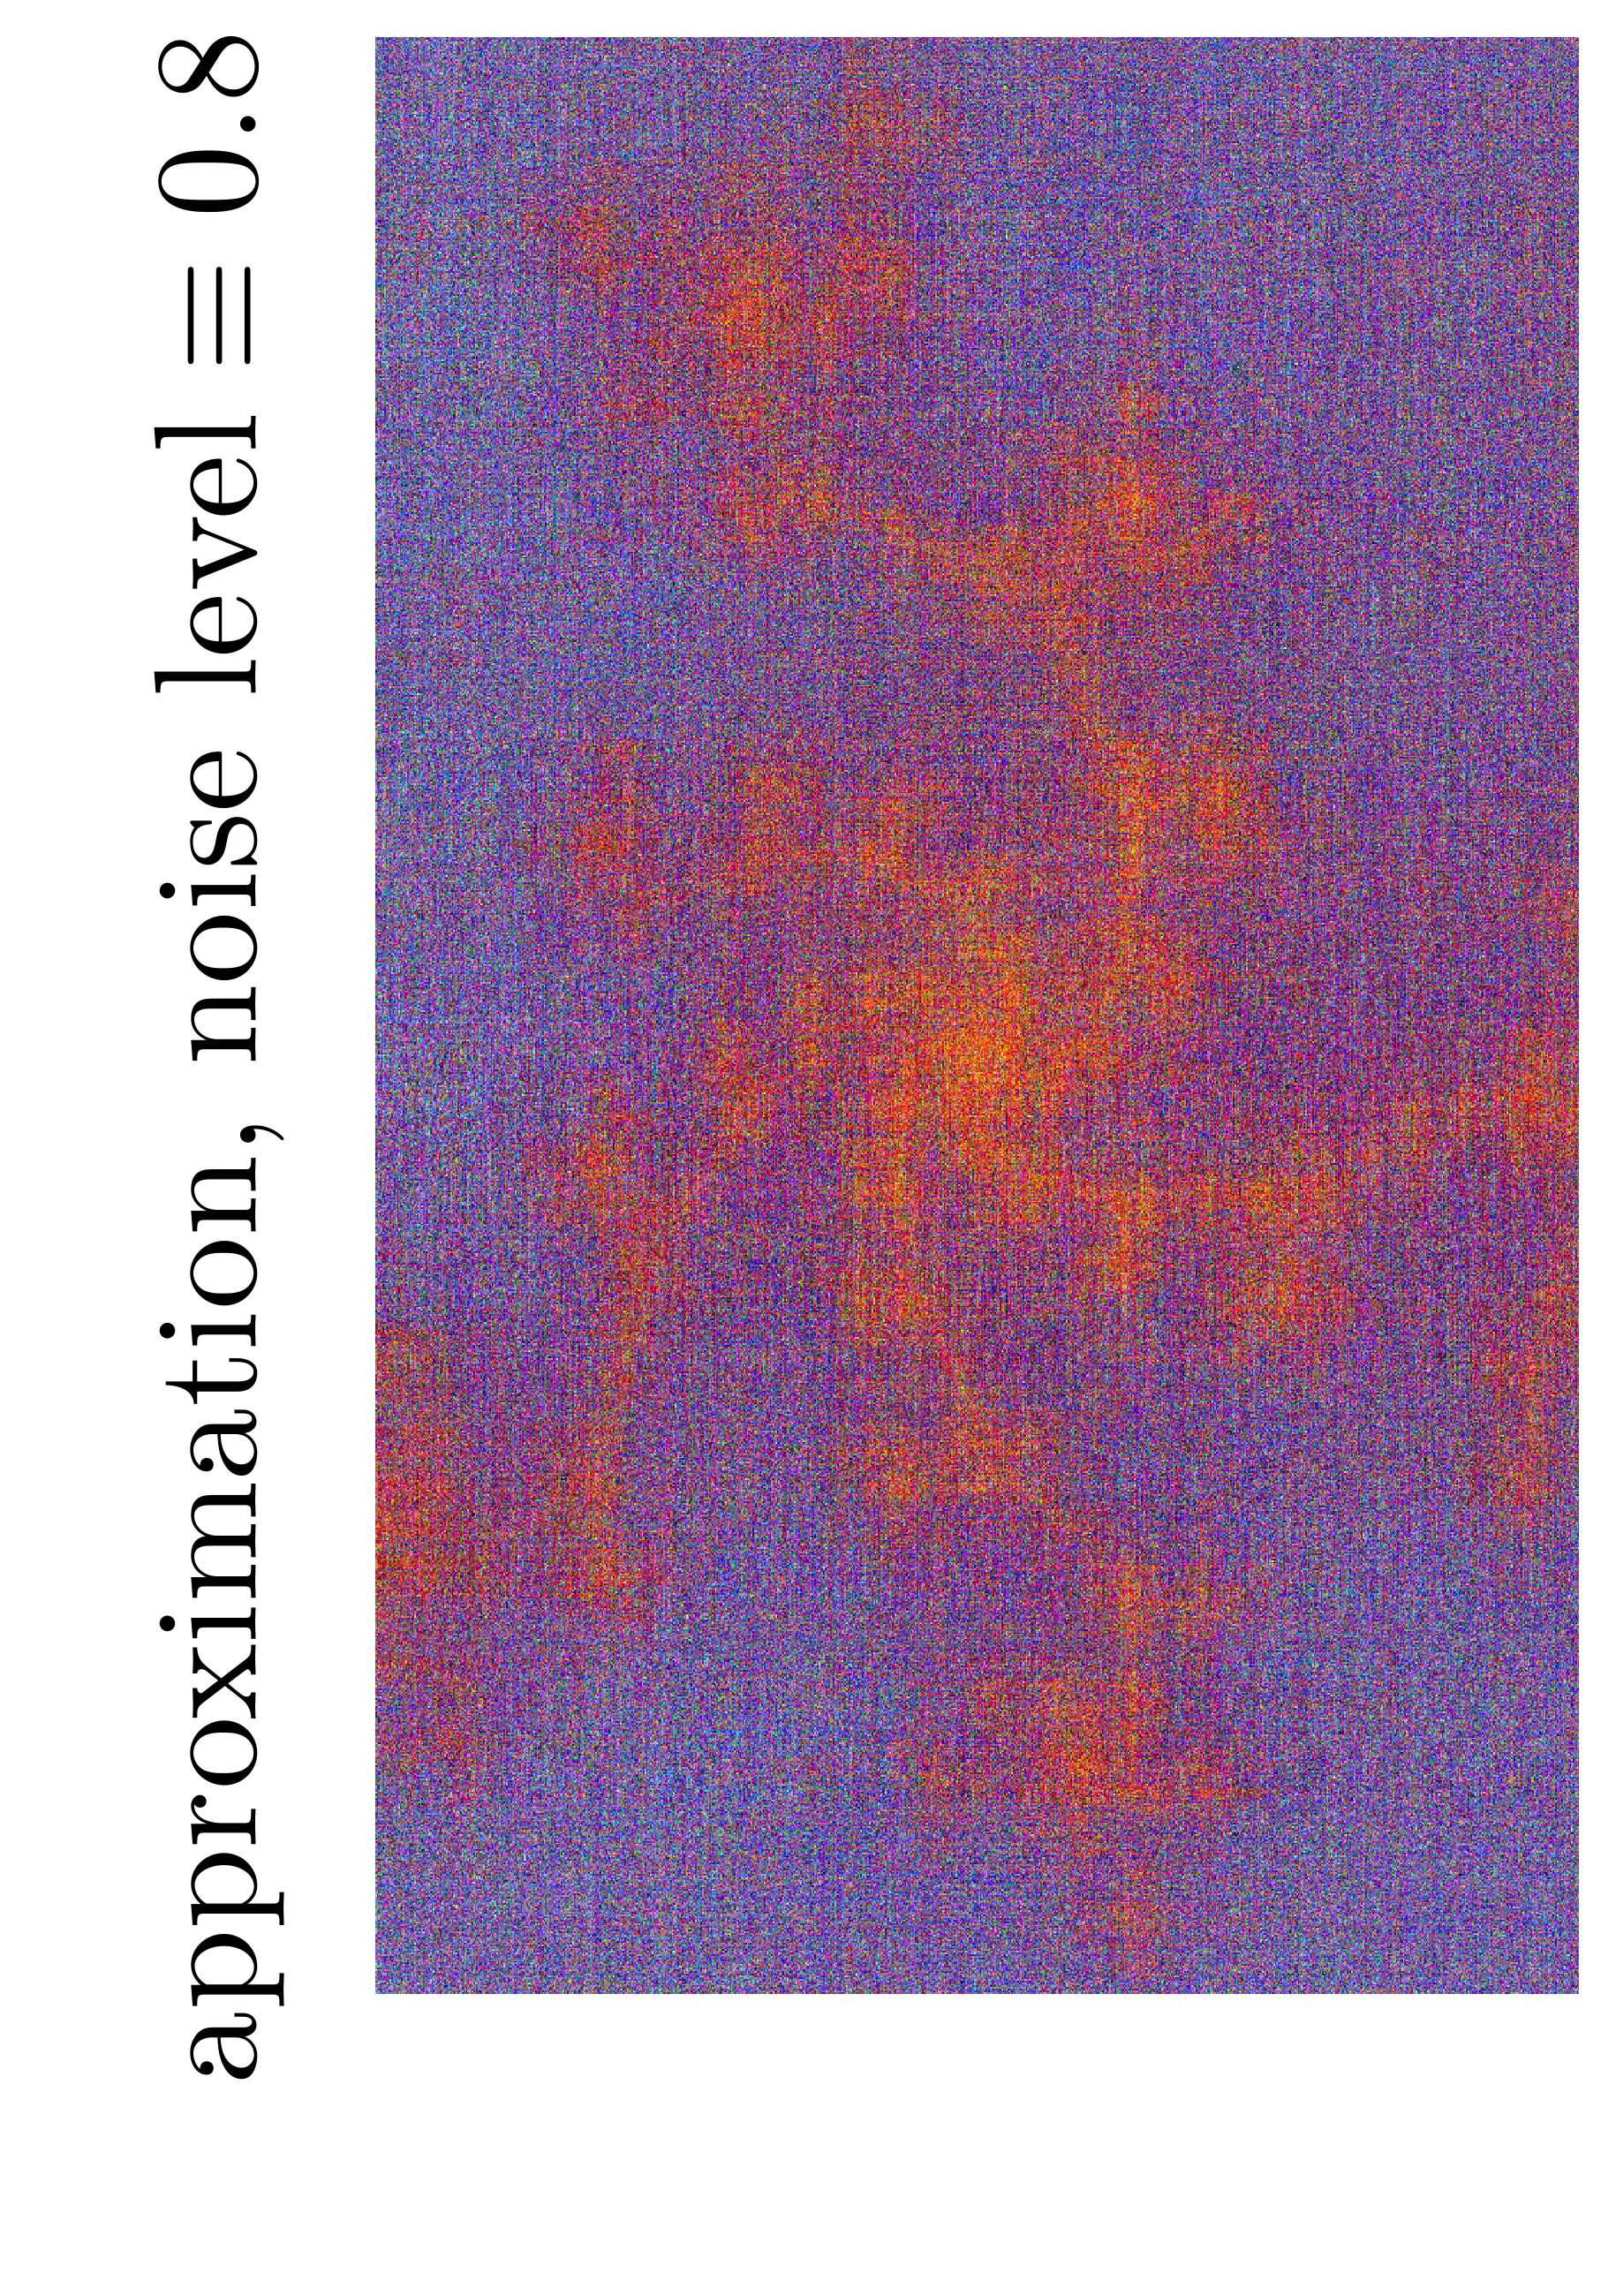
\includegraphics{figures/mandelbrot_noise_approx6.png}}
    \caption{(a) SVD of an image of a portion of the Mandelbrot set, mixed with different levels of white noise (black to bright gray: $0$, $0.2$, $0.4$ and $0.8$), plotted in panels (b,d-f).
    The original picture shows a fast decay of the Schmidt values compared to the higher noise levels, leading to a reasonable approximation (compare panel (b) with panel (c)). The amount of noise alters the algebraic decay of the Schmidt values, ultimately resulting in a larger error, and more noticeable deviations to the original picture (compare panels (d-f) with panels (g-i)). The number of Schmidt values kept in the approximations is fixed to $100$.}
    \label{fig:svd_image_compression_mandelbrot}
\end{figure}

The depicted compression scheme can actually be applied to quantum states.
Recall that any state can be expressed by a set of $L$ good quantum numbers, such that
\begin{align}
    \ket{\psi} = \sum_{i_1,i_2,\dots,i_L}C({i_1,i_2,\dots,i_L})\ket{i_1,i_2,\dots,i_L}
    \label{eq:generic_state}
\end{align}
and the collection of all $\ket{i_1,i_2,\dots,i_L}$ form a complete and orthonormal basis.
Note that the $L$-dimensional array $C$ depends on all internal quantum numbers and is thus exponentially large in the system size $L$ and the dimension of the quantum numbers $i_j$.
By the visual conventions, we may imagine the coefficients $C$ as a rank $L$ tensor, similar to the tensor $T$ discussed in \cref{eq:SVD_generalized}, i.e.
\begin{align}
    C(i_1,i_2,\dots,i_L) \rightarrow C^{[i_1,i_2,\dots,i_L]} \equiv  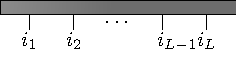
\includegraphics[valign=c]{figures/arbitrary_wavefunction.pdf}.
\end{align}
To account for the fact that the indices ${\bm i} = i_1,i_2,\dots,i_L$ are not fixed to specific values here, we will from now on denote the dependence of the tensor $C$ on the set of quantum numbers with square brackets.
We now proceed by applying the generalized SVD in a sequential manner:
Starting with the decomposition spanned by the bipartition of the first (last) leg, keeping the left (right) isometry and shifting the right (left) isometry to the adjacent leg position, is possible to decompose $C$ into a product of isometries with a single matrix in between two arbitrary leg positions $\ell,\ell+1$.
The decomposition sequence is easily reformulated in graphical notation
\begin{align}
    C^{[i_1,i_2,\dots,i_L]} \equiv 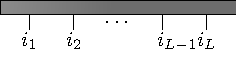
\includegraphics[valign=c]{figures/arbitrary_wavefunction.pdf},
    =
    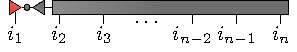
\includegraphics[valign=c]{figures/arbitrary_wavefunction_partially_decomposed_1.pdf},
    \\
    =
    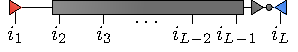
\includegraphics[valign=c]{figures/arbitrary_wavefunction_partially_decomposed_2.pdf},
    \\
    =
    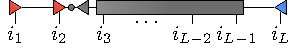
\includegraphics[valign=c]{figures/arbitrary_wavefunction_partially_decomposed_3.pdf},
    \\
    =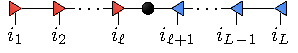
\includegraphics[valign=c]{figures/arbitrary_wavefunction_decomposed.pdf},
    \label{eq:move_the_lambda_matrix}
\end{align}
in which at each step the three gray tensors are contracted before performing the next SVD.
This particular decomposition of a generic quantum state, i.e.
\begin{align}
    C^{[i_1,i_2,\dots,i_L]} \equiv 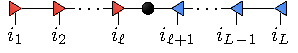
\includegraphics[valign=c]{figures/arbitrary_wavefunction_decomposed.pdf},
    \label{eq:mixed_canonical_form}
\end{align}
is called the (mixed) canonical form of an MPS\footnote{One could even perform the sequence \cref{eq:move_the_lambda_matrix} by leaving the Schmidt weights on every link, thus obtaining another canonical form -- the so-called $\Gamma-\lambda$ form~\cite{Vidal2007,Orus2008}.}.
In other words, it represents the Schmidt decomposition of the state $\ket{\psi}$ in the subspaces $\HS_{A(\ell)}$ and $\HS_{B(\ell)}$ spanned by the first $\ell$ and last $L-\ell$ quantum numbers i.e.
\begin{align}
    \ket\psi = \sum_{\bm i} C^{[\bm i]}\ket{\bm i} = \sum_{k}s_{k}(\ell)\ket{\psi_{A(\ell),k}}
    \ket{\psi_{B(\ell),k}},
    \label{eq:schmidt_decomposition}
\end{align}
in which the transformed states $\ket{\psi_{A/B,k}}$ are given by the SVD-decomposed coefficient tensor
\begin{align}
    \ket{\psi_{A(\ell),k}}
    &=
    U^{[i_1]}_{k_1} U^{[i_2]}_{k_1,k_2}U^{[i_3]}_{k_2,k_3}\dots U^{[i_\ell]}_{k_{\ell-1},k}\ket{i_1,i_2,i_3,\dots,i_j}
    =\prod_{k=1}^\ell U^{[i_k]}\ket{i_1,\dots,i_\ell},\\
    %
    \ket{\psi_{B(\ell),k}}
    &=
    {V^\dag}^{[i_{\ell+1}]}_{k,k_{\ell+1}} {V^\dag}^{[i_{\ell+2}]}_{k_{\ell+1},k_{\ell+2}}\dots {V^\dag}^{[i_L]}_{k_{L-1}}\ket{i_{\ell+1},\dots,i_L}
    =
    \prod_{k=\ell+1}^L V^{\dag[i_k]}\ket{i_{\ell+1},\dots,i_L}.
    \label{eq:bipartition_orthonormal_basis}
\end{align}
In the two expressions above, we conveniently use the sum convention.
Note that the position of the central matrix in \cref{eq:mixed_canonical_form} is not fixed to the center of the chain.
It can be moved arbitrarily to the right (left) by a sequence of singular value decompositions
\begin{align}
    \Lambda(\ell) V^{\dag[i_{\ell+1}]}V^{\dag[i_{\ell+2}]} &= U^{[i_{\ell+1}]}\Lambda(\ell+1) \tilde V^{\dag[i_{\ell+1}]}
    \equiv
    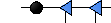
\includegraphics[valign=c]{figures/fMPS_3_1.pdf}
    =
    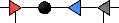
\includegraphics[valign=c]{figures/fMPS_3_2.pdf},
    \\
    U^{[i_{\ell-1}]}U^{[i_{\ell}]}\Lambda(\ell) &= \tilde U^{[i_{\ell-1}]}\Lambda(\ell-1) \tilde V^{\dag[i_{\ell}]}
    \equiv
    
\includegraphics[valign=c]{figures/fMPS_4_1.pdf}
    =
    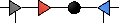
\includegraphics[valign=c]{figures/fMPS_4_2.pdf}.
\end{align}
Due to its fundamental importance for the remaining section, we will from now on use the notation
\begin{align}
    \ket\psi = \brlr{\prod_{k=1}^\ell U^{[i_k]}}\Lambda(\ell)\brlr{\prod_{k=\ell+1}^L V^{\dag[i_k]}}\ket{i_1,i_2,\dots,i_L}
\end{align}
to denote the mixed canonical decomposition of the coefficient tensor $C$ with rank-$3$ isometries ${U^{[i_k]}/V^{\dag[i_k]}}$ and a matrix $\Lambda(\ell)$ containing the Schmidt values of the bipartition after site $\ell$.
It is now obvious that (i) any quantum state can be decomposed into an MPS, (ii) that each MPS can be brought into the mixed canonical form and (iii) that MPS have a large gauge degree of freedom.
Point (iii) is clear from the fact that one may sandwich infinitely many identities in the MPS (each written as a product of two unitary matrices) which may in general rotate the colored isometry tensors, but leave the overall state invariant.
%
%
%%%%%%%%%%%%%%%%%%%%%%%%%%%%%%%%%%%%%%%%%%%%%%%%%%%%
\section{Reduced density matrix and Rényi entropy}
\label{sec:reduced_density_matrix_and_renyi_entropy}
%%%%%%%%%%%%%%%%%%%%%%%%%%%%%%%%%%%%%%%%%%%%%%%%%%%%
%
%
To understand the influence of the compression scheme, consider the density matrix of an MPS in canonical form:
\begin{align}
    \hat\rho = \sum_{k,k'}s_ks_{k'}\ket{\psi_{A,k},\psi_{B,k}}\bra{\psi_{A,k'},\psi_{B,k'}}.
\end{align}
Now imagine to compute the reduced density matrix of a bipartition formed by a block $A(\ell)$ of the first $\ell$ quantum numbers and a block $B(\ell)$ of the remaining ones.
A trace over the complement states of the partition $A/B$ gives the reduced density matrix in block $A/B$, i.e.
\begin{align}
    \hat\rho_A = \tr_B(\hat\rho)
    &=
    \sum_{k,k',k''}
    s_ks_{k'}
    \braket{\psi_{B,k''}|\psi_{A,k},\psi_{B,k}}\braket{\psi_{A,k'},\psi_{B,k'}|\psi_{B,k''}}
    =
    \sum_k s_k^2 \ket{\psi_{A,k}}\bra{\psi_{A,k}},\nonumber\\
    %
    \hat\rho_B = \tr_A(\hat\rho)
    &=
    \sum_k s_k^2 \ket{\psi_{B,k}}\bra{\psi_{B,k}}.
\end{align}
Note that normalization of the quantum state $\ket\psi$ implies $\tr\rho=\sum_k s_k^2=1$ and $s_k^2$ can be interpreted as the probability of state $\ket{\psi_{A/B,k}}$ contributing to the reduced density matrix $\hat\rho_{A/B}$.
The reduced density matrix is thus diagonal in the Schmidt decomposition, and solely determined by the spectral values $s_k$.
Imagine now to approximate the state $\ket\psi$ with a state $\ket{\psi'}$ by limiting the number of different $s_k$ in the bipartition $A,B$ such that the $m$ largest spectral values are kept in $\ket{\psi'}$ and the rest is set to zero.
Normalization of the state $\ket{\psi'}$ requires that $\sum_{k=1}^m {s'_k}^2$ must be renormalized to unity, which is satisfied if $s_k'=s_k/\sqrt{\sum_{l=1}^m s_l^2}$.
The threshold $m$ is thus directly related to approximating the reduced density matrix $\hat \rho_{A/B}$ with the $m$ most likely states in the Schmidt decomposition of a given bipartition $A/B$.
Please note that $s_k\equiv s_k(\ell)$ refers to the $k$'th singular value of a particular bipartition $A(\ell)/B(\ell)$, which considers the first/last $\ell/L-\ell$ quantum numbers.
% Therefore, it can be appropriate to denote this dependence also in the spectral values if needed, i.e. $s_k = s_k(\ell)$.
If we keep the $m$ largest singular values $s_k(\ell)$, $k\in\{1,2,\dots,m\}$ for any block size $\ell$, $m$ is a global property of MPS called the bond dimension.

Density matrices are naturally related to the generalized Gibbs entropy for quantum states
\begin{align}
    S_1(\ell) = -\tr(\hat\rho_A\log\hat\rho_A) = -\tr(\hat\rho_B\log\hat\rho_B) = -\sum_k s^2_k\log(s^2_k)
\end{align}
which is a straightforward measure for the shared information between the bipartition, in information theory perspectives often called Shannon entropy of communication.
In this context, $-\log(s^2_k)$ is understood as the information content (or surprisal) of the Schmidt state, and $S_1$ is simply the expectation value of surprisal.
Such a definition is understood intuitively: measuring a state of very low probability is surprizing, whereas likely quantum states bear a low surprise.
In a quantum physics audience, the entropy $S_1$ is commonly referred to as von Neumann entropy, and we denote it as $S_1$ because of its relation to the Rényi entropy -- a generalized version of the Shannon entropy
\begin{align}
    S_\alpha(\ell) = \frac{1}{1-\alpha}\log\tr\hat\rho^\alpha_A
\end{align}
in the limit $\alpha\rightarrow1$.
The derivation of the limit is infrequently presented in the literature, but straightforward by using the Schmidt decomposition and L'Hôpital's rule
\begin{align}
    S_1(\ell)
    =
    \lim_{\alpha\rightarrow1}\frac1{1-\alpha}\log\tr\hat\rho_A^\alpha
    =
    -\lim_{\alpha\rightarrow1}\partial_\alpha\log\sum_k s_k^{2\alpha}
    =
    -\lim_{\alpha\rightarrow1}\frac{\sum_k\partial_\alpha s_k^{2\alpha}}{\sum_k s_k^{2\alpha}}
    =
    -\lim_{\alpha\rightarrow1}\sum_k \partial_{\alpha}\re^{\alpha\log s_k^2}
    \\
    =
    -\lim_{\alpha\rightarrow1}\sum_k \re^{\alpha\log s_k^2}\log s_k^2
    =
    -\sum_k s_k^2\log s_k^2
    =
    -\tr \hat\rho_A\log\hat\rho_A.
\end{align}
In conclusion, using MPS techniques in the canonical form provides immediate access to the information content of a given bipartition.
Note that the maximum entropy of an MPS is always restricted by the bond dimension $m$, i.e. $S_1(\ell)<\log(m)$.
%
%
%%%%%%%%%%%%%%%%%%%%%%%%%%%%%%%%%%%%%%%%%%%%%%%%%%%%%%%%%
\section{Scaling relations of the entanglement entropy}
\label{sec:scaling_relations_of_the_entanglement_entropy}
%%%%%%%%%%%%%%%%%%%%%%%%%%%%%%%%%%%%%%%%%%%%%%%%%%%%%%%%%
%
%
All of the discussion so far would not be very exciting for a wholehearted physicist, were it not for its close relation to quantum entanglement.
The phenomenon was firstly noted in $1935$ by Albert Einstein, Boris Podolsky, and Nathan Rosen~\cite{EPR1935}, also by Erwin Schrödinger~\cite{Schrdinger1935,Schrdinger1936}, describing what is famously known as the EPR paradox~\cite{Reid2009}.
At its heart, it describes a group of particles interacting such that the quantum state of each individual particle cannot be described independently of the state of the others in the group.
The paradox part in the aforementioned works is described by quantum measurements performed on individual particles, which leads to irreversible collapses of the wave function and an alteration of the original quantum state of the other particles in the group.
Surprisingly, the phenomenon is independent of the distance between the particles and forms thus a unique form of correlations exclusively present in quantum systems.

To make an example, consider the two-particle pure state $\ket{\psi}=\frac1{\sqrt2}\brlr{\ket{\uparrow\downarrow}+\ket{\downarrow\uparrow}}$ and the two particles being localized at two distant spacial positions.
In case we prepare a projective measurement of the first particle being in the $\uparrow$-state, the probability of the outcome is obviously $1/2$ and we end up with a collapsed post-measurement state of the form $\ket{\tilde\psi} = \ket{\uparrow\downarrow}$.
At the time of the measurement, the second particle collapses to the perfectly correlated alignment, and it does so immediately, independent on the spacial distance between the two parties.
A subsequent measurement of the second particle will thus yield $\downarrow$ with probability $1$.
Note that this instantaneous action does not violate causality since the outcome of the first measurement is random and as such cannot be used to transmit information\footnote{Until the outcome of the first measurement is communicated, the density matrix of the second spin is that of a mixed state, i.e. $1/2$ times the identity.}.
With this example in mind, let us now encapsulate the definition of $N$-partite separable and entangled for states with $N$ individual particles.

A state $\ket{\psi}$ is called $N$-partite separable iff. it can be written as a product of $N$ subsystems~\cite{Horodecki2009}
\begin{align}
    \ket{\psi} = \ket{\psi_1}\otimes\ket{\psi_2}\otimes\dots\otimes\ket{\psi_N}.
    \label{eq:separable_states}
\end{align}
Note that this expression is fundamentally different from the coherent superposition of exponentially many state vectors encountered in generic states (compare to ~\cref{eq:generic_state}).
As such, we call a state $N$-partite entangled, if it cannot be decomposed according to~\cref{eq:separable_states}.
The earlier example of a bipartite system is an element of the Bell basis, which are sometimes called EPR states
\begin{align}
    \ket{\psi^\pm}=\frac 1{\sqrt2}\brlr{\ket{\uparrow\downarrow}\pm\ket{\downarrow\uparrow}}
    \quad
    \ket{\phi^\pm}=\frac 1{\sqrt2}\brlr{\ket{\uparrow\uparrow}\pm\ket{\downarrow\downarrow}}
\end{align}
and they all have remarkable properties, first recognized by Schrödinger -- if one measures only one of the states, one finds it with equal probability in either $\ket{0}$ or $\ket{1}$.
As such, they give no information about the subsystems, whereas they are still pure and thus reveal full information about the global system.
The Bell states are special cases of bipartite maximally entangled states~\cite{Horodecki2009} and as such great examples to explore the entropic manifestation of entanglement.

In particular, the von Neumann entropy of a product state vanishes\footnote{This is actually a consequence of a much more general statement for open quantum systems and mixed states: the entropy of a subsystem can be greater than the entropy of the global system iff. the state is entangled~\cite{Horodecki1994}.
The inequality for separable states can thus be expressed as $S(\hat\rho)-S(\hat\rho_{A/B})\geq0$ with $\hat\rho$ the density matrix of the mixed state and $\hat\rho_{A/B}$ the reduced density matrix of bipartition $A/B$.
As such, the von Neumann entropy serves as a scalar separability criteria, in analogy to the Bell inequalities~\cite{Horodecki2006}.}.
Note that the reduced density matriy of the Bell states is $\hat\rho_{A/B}=\frac12\mathbb1$ and as such $S_1=\log2$ which provides an upper limit for this two-partite system.
In general, a maximally entangled $N$-partite pure state is maximally entangled if the reduced density matrix is proportional to the identity.
Assuming the local internal dimension is $D$, it assumes the upper bound of the entropy $S_1(\ell)=\ell\log(D)$.
On the contrary, a product state has vanishing entropy.

Coming back to the connection to MPS with finite bond dimension, we now know that the upper bound restriction of the entropy limits the available entanglement of the approximation.
This, in turn, does not provide an explanation why such an approximation should not ``go wrong quickly'' in a sense that the important properties of the approximated state are lost, even if the bond dimension is large.
Incidentally, at the time DMRG was introduced by Steven White~\cite{White1992}, the success of the renormalization scheme remained a mystery.
Some insights were concluded by the derivation of universal scaling laws of the entropy provided e.g. by Calabrese and Cardy in 2004~\cite{Calabrese2004} in proximity of a quantum critical point.
In 2007, Hastings published his famous proof of the area law for one-dimensional quantum systems~\cite{Hastings2007}.
In its essence, it provides an upper bound to the von Neumann entropy for gapped and local (i.e. no long-ranged interactions) Hamiltonians scaling as the area ($\equiv$ a constant) of one-dimensional systems.
Essentially, the works can be summarized by the following two statements~\cite{Eisert2010}:
Consider a block of $1,2,\dots,\ell$ sites in a system of $N$ sites in total, then the entanglement entropy of the physically relevant part (i.e. the low-energy/temperature subspace of $\HS$) scales as
\begin{align}
    S_1(\ell) &=
    \frac c{3b}
    \left\{
    \begin{array}{l}
        \log[d(\ell)],\text{ if the system is gapless, and if $N\gg\ell\gg 1$,}\\[0.25cm]
        \log[\xi/a],\,\text{ if the correlation length $\xi$ is finite, and if $N\gg\ell\gg\xi/a$.}
    \end{array}
    \right.
    \label{eq:entropy_scaling}
\end{align}
In the above, $b$ encodes periodic ($b=1$) and open ($b=2$) boundary conditions, $c$ is the central charge of the conformal field theory (in a fermionic model, it corresponds to the number of Fermi momenta) and $d(\ell)$ is the ``chord distance'', which describes the length of a semi-circle
\begin{align}
    d(\ell) = \left|\frac{N}{\pi}\sin(\pi\ell/N)\right|.
\end{align}
The main message of \cref{eq:entropy_scaling} is that, for gapped systems, physically relevant states live in the low-entangled subspace of the full Hilbert space.
This implies that the MPS Ansatz is an optimal choice to target the low-lying excitations of the full many body Hilbert space, which, in turn, follow an area law of entanglement.

The generalization of MPS to higher dimensional lattices are called projected entangled pair states (PEPS), which, like the MPS, have the area law already built into their very construction.
In particular, they satisfy $S(\rho_A)=\mathcal O(|\partial A|)$ in which $\partial A$ denotes the boundary area of any subset $A$ of lattice sites.
Although a general proof as in the case of 1D gapped Hamiltonians is presently not established, area laws have been proven for non-interacting and gapped models (both bosonic and fermionic), and have also been checked vor various strongly correlated interacting systems~\cite{Eisert2010,Laflorencie2016}.
%
%
%%%%%%%%%%%%%%%%%%%%%%%%%%%%%%%%%%%%
\section{Matrix product operators}
\label{sec:matrix_product_operators}
%%%%%%%%%%%%%%%%%%%%%%%%%%%%%%%%%%%%
%
%
Let us now understand the action of operators in the basis of MPS.
Consider a local operator acting on site $q$, which can be written in general as $\hat o_q = \sum_{i_q',i_q''}o_{i_q',i_q''}\ket{i_q'}\bra{i_q''}$.
Its action on the canonical form of an MPS can be expressed as
\begin{align}
    \hat o_q\ket\psi &= \sum_{i_1,i_2,\dots,i_q,\dots,i_L}\sum_{i_q'}o_{i_q',i_q} C^{i_1,i_2,\dots,i_q,\dots,i_L}\ket{i_1,i_2,\dots,i_{q-1},i_q',i_{q+1},\dots,i_L}
    \\
    &= \sum_{i_1,i_2,\dots,i_L}\tilde C^{i_1,i_2,\dots,i_L}\ket{i_1,i_2,\dots,i_L}
\end{align}
and we note that it leaves the overall form of the MPS invariant.
In particular, it acts as a contraction between the $o$-matrix and the $q$'th vertical leg of the $C$-tensor, according to
\begin{align}
    \tilde C^{i_1,i_2,\dots,i_q,i_{q+1},\dots,i_{L-1},i_L} = \sum_{i_q'}o_{i_q,i_q'}C^{i_1,i_2,\dots,i_q',i_{q+1},\dots,i_{L-1},i_L}\equiv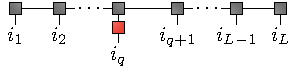
\includegraphics[valign=c]{figures/operator_mps.pdf}.
\end{align}
Therefore, we can represent any local operator as a rank-$2$ tensor composed by the matrix elements of $\hat o$.
The same reasoning applies for operators acting on $p$ sites -- they are represented by rank-$2p$ tensors containing the entries of the matrix elements, contracted with the $p$ corresponding vertical links of the $C$-tensor.

The most straightforward example of a matrix product operator is given through the Hamiltonian, and the derivation straightforward.
Consider for example the Ising model
\begin{align}
    \hat H = \hat H_{h} + \hat H_{J},
    \quad
    \hat H_{J} = J\sum_{i=\ell}^{L-1}\hat X_\ell \hat X_{\ell+1},
    \quad
    \hat H_{h} = h\sum_{\ell=1}^{L}\hat Z_\ell,
\end{align}
in which $\hat X/\hat Y/\hat Z$ denote the spin-1/2 operators.
They have the following representations
\begin{align}
    \hat X_\ell/\hat Y_\ell/\hat Z_\ell = \sum_{i_\ell,i'_\ell\in\{\uparrow,\downarrow\}}X_{i_\ell,i_\ell'}/Y_{i_\ell,i_\ell'}/Z_{i_\ell,i_\ell'}\ket{i_\ell}\bra{i'_\ell},
\end{align}
in which $X/Y/Z$ are the spin-1/2 Pauli matrices
\begin{align}
    X =
    \begin{pmatrix}
        0 & 1 \\
        1 & 0
    \end{pmatrix}
    ,
    \quad
    Y =
    \begin{pmatrix}
        0 & -\ri \\
        \ri & 0
    \end{pmatrix}
    ,
    \quad
    Z =
    \begin{pmatrix}
        1 & 0 \\
        0 & -1
    \end{pmatrix}.
\end{align}
The additional subscript $\ell$ denotes an isolated action of $\hat X_\ell/\hat Y_\ell/\hat Z_\ell$ on the $\ell$'th spin of the system.

Note that the Hamiltonian can be recast into a product of operators according to
\begin{align}
    \hat H = \hat W_1\brlr{\prod_{\ell=2}^{L-1}\hat W_{\ell}}\hat W_L,
\end{align}
in which we conveniently use a set of bulk $\hat W_{\ell\neq1,L}$, and two additional boundary operators $\hat W_1$, $\hat W_L$.
The bulk operators have the form
\begin{align}
    \hat W_{\ell\neq1,L} =
    \begin{pmatrix}
        \hat{\mathbb 1}_\ell & \hat X_\ell & h \hat Z_\ell\\
         0 & 0 & J \hat X_\ell\\
        0 & 0 & \hat{\mathbb 1}_\ell\\
    \end{pmatrix}
\end{align}
representing a set of local operators acting locally on a single site $\ell$.
Similarly, the boundary operators are given by
\begin{align}
    \hat W_1 =
    \begin{pmatrix}
        1 & 0 & 0
    \end{pmatrix}
    \begin{pmatrix}
        \hat{\mathbb 1}_1 & \hat X_1 & h \hat Z_1\\
        0 & 0 & J \hat X_1\\
        0 & 0 & \hat{\mathbb 1}_1\\
    \end{pmatrix}
    =
    \begin{pmatrix}
        \hat{\mathbb 1}_1 & \hat X_1 & h \hat Z_1
    \end{pmatrix}
    ,
    \quad
    \hat W_L =
    \begin{pmatrix}
        \hat{\mathbb 1}_L & \hat X_L & h \hat Z_L\\
        0 & 0 & J \hat X_L\\
        0 & 0 & \hat{\mathbb 1}_L\\
    \end{pmatrix}
    \begin{pmatrix}
        0 \\ 0 \\ 1
    \end{pmatrix}
    \begin{pmatrix}
        h \hat Z_L\\
        J \hat X_L\\
        \hat{\mathbb 1}_L\\
    \end{pmatrix}.
    \label{eq:boundary_W}
\end{align}
Since $\hat W_\ell$ spans a matrix with entries composed of local operators, which each have an MPO representation, the action of the Hamiltonian on a state $\ket\psi$ can be understood as a product of rank-$4$ tensors $W^{[i_\ell',i_\ell]}$ containing the matrix elements of $\hat W_{\ell}$.
In particular, one obtains the following tensorial representation, acting on a single site $\ell\neq1,L$ of the bulk
\begin{align}
    W^{[i_\ell',i_\ell]} =
    \begin{pmatrix}
        \delta_{i_\ell',i_\ell} & X_{i_\ell',i_\ell} & h Z_{i_\ell',i_\ell} \\
        0 & 0 & J X_{i_\ell',i_\ell} \\
        0 & 0 & \delta_{i_\ell',i_\ell}
    \end{pmatrix}
    \equiv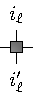
\includegraphics[valign=c]{figures/mpo.pdf}
    .
\end{align}
It is straightforward to introduce two additional boundary tensors, in equivalence to \cref{eq:boundary_W}
\begin{align}
    W^{[i_1',i_1]} =
    \begin{pmatrix}
        \delta_{i_1',i_1} & X_{i_1',i_1} & h Z_{i_1',i_1}
    \end{pmatrix}
    \equiv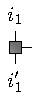
\includegraphics[valign=c]{figures/mpo_left.pdf}
    ,\quad
    W^{[i_L',i_L]} =
    \begin{pmatrix}
         h Z_{i_L',i_L} \\
         J X_{i_L',i_L} \\
         \delta_{i_L',i_L}
    \end{pmatrix}
    \equiv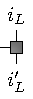
\includegraphics[valign=c]{figures/mpo_right.pdf}.
\end{align}
The MPO representation of the Hamiltonian is quite versatile -- any Hamiltonian can be recast into a set of matrix product operators that are upper triangular (or lower triangular), even if the interactions are long-ranged or spatially dependent, e.g. in the case of disorder.
Note that the MPO form is not limited to spin systems due to the famous Jordan-Wigner transformation.
It is defined in terms of the ladder operators with matrix representations $\hat\sigma^\pm = \frac12(\hat X\pm\ri \hat Y)$, i.e.
\begin{align}
    \hat c_i^\pdag = \brlr{\prod_{j<i}-\hat Z}\hat\sigma^-_i,
    \qquad
    \hat c_i^\dag = \brlr{\prod_{j<i}-\hat Z}\hat\sigma^+_i.
    \label{eq:jordan_wigner_trafo}
\end{align}
This way, the fermionic creation and annihilation operators are represented by spin ladder operators.
To restore the anticommutation relations of fermions, the additional phase string is required.
Note that the presence of the string of $\hat Z$'s in general imposes long-ranged interactions in two-dimensional systems, such that a direct application of the Jordan-Wigner transformation is primarily used in (quasi-)one-dimensional systems~\cite{Franchini2017}\footnote{For higher-dimensional lattices, the Bravyi-Kitaev mapping may be more suited~\cite{Bravyi2002}.}.
%
%
%%%%%%%%%%%%%%%%%%%%%%%%%%%%%%%%%%%%%%%%%%%
\section{Variational ground state search}
\label{sec:variational_ground_state_search}
%%%%%%%%%%%%%%%%%%%%%%%%%%%%%%%%%%%%%%%%%%%
%
%
The original variational ground state search is formalized in the density matrix renormalization group (DMRG), introduced by Steven White in 1992~\cite{White1992}.
In it's essence, it is a numerical optimization scheme targetting the low energy sector of a given system.
Nowadays, it is understood as an MPS Ansatz of the trial wavefunction in which at each iteration a few local tensors (in most cases one or two) are variationally optimized.
For the numerical simulations employed in all of our articles, we implemented two optimization schemes, which are then combined to find an optimal MPS approximation for finite systems.
The first one is the growing algorithm (sometimes dubbed iDMRG), which is most useful to construct the trial wavefunction of the second scheme, namely traditional DMRG reformulated in the language of MPS~\cite{Schollwoeck2011,Silvi2019}.

Consider the way the energy expectation value is written in the MPS language: it is a sandwich of the product of $W$ tensors (the local MPO representing the Hamiltonian) with the trial MPS, and it's conjugate.
To find the groundstate, we extremize the energy
\begin{align}
    E = \min_{\ket{\psi}}\braket{\psi |\hat H | \psi}
\end{align}
under the constraint that $\braket{\psi|\psi}=1$.
Using a Lagrange multiplier, the equation becomes
\begin{align}
    \braket{\psi|\hat H|\psi} - \lambda_\psi\brlr{\braket{\psi|\psi}-1} = 0.
    \label{eq:lagrangian_multiplier}
\end{align}
Now the MPS structure of $\ket\psi$ is exploited, and we decompose the state into the canonical form
\begin{align}
    \ket\psi
    =
    \brlr{\prod_{k=1}^{\ell}U^{[i_k]}}\Lambda(\ell)\brlr{\prod_{k=\ell+1}^{L}V^{\dag[i_k]}}\ket{\bm i}
    \equiv
    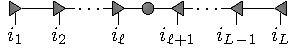
\includegraphics[valign=c]{figures/arbitrary_wavefunction_decomposed_decolorized.pdf}\ket{i_1,i_2,\dots,i_L}.
\end{align}
Please note that we use the sum convention in the above, and the tensors $U^{[i_k]}$ and $V^{\dag[i_k]}$ satisfy the isometry conditions
\begin{align}
    \sum_{i_k}U^{\dag[i_k]}U^{[i_k]} = \mathbb 1,
    \quad
    \sum_{i_k}V^{\dag[i_k]}V^{[i_k]} = \mathbb 1.
    \label{eq:isometry_tensors}
\end{align}
Diagrammatically, the two conditions exactly correspond to the two graphical contractions
\begin{align}
    \includegraphics[valign=c]{figures/left_isometry_tensor.pdf}
    =
    \includegraphics[valign=c]{figures/identity_tensor_left.pdf}\,,
    \quad
    \includegraphics[valign=c]{figures/right_isometry_tensor.pdf}
    =
    \includegraphics[valign=c]{figures/identity_tensor_right.pdf}\,.
    \label{eq:isometry_tensors_diagram}
\end{align}
To cast \cref{eq:lagrangian_multiplier} into a variational problem for the tensors at position $\ell$ and $\ell+1$, it is convenient to use the graphical notation
\begin{align}
    \includegraphics[valign=c]{figures/lagrangian_multiplier_equation_1.pdf}
    -
    \lambda_\psi
    \brlr{\includegraphics[valign=c]{figures/lagrangian_multiplier_equation_2.pdf}-1}
    =
    0.
    \label{eq:lagrangian_multiplier_graphical}
\end{align}
In the above, we use square tensors to denote the local MPOs of the Hamiltonian.
The aim is now to optimize all tensors in order to extremize \cref{eq:lagrangian_multiplier_graphical}.
To obtain something feasible, we now derive an equation which considers a local optimization of the two colored tensors.
This is achieved by the application of a gradient on both sides of \cref{eq:lagrangian_multiplier}, in which we derive with respect to the entries of the contraction of the red, black and blue tensor, i.e.
\begin{align}
    \nabla(\ell,\ell+1)_{kn}\equiv\frac\partial{\partial\brlr{U^{i_\ell}_{k,l}S_l V^{\dag i_{\ell+1}}_{l,n}}^*}.
\end{align}
Since the tensors enter in the equation in a linear fashion, the application of the gradient simply corresponds to removing the three tensors from the conjugate contraction (and of course the scalar $1$) in \cref{eq:lagrangian_multiplier_graphical}.
One arrives at the tensorial expression
\begin{align}
    \includegraphics[valign=c]{figures/lagrangian_multiplier_equation_3.pdf}
    =
    \lambda_\psi
    \includegraphics[valign=c]{figures/lagrangian_multiplier_equation_4.pdf}
    .
    \label{eq:lagrangian_multiplier_graphical_2}
\end{align}
This can be better understood after reshaping $U^{[i_\ell]}\Lambda(\ell) V^{\dag[i_{\ell+1}]}$ (the red, black and blue tensors in \cref{eq:lagrangian_multiplier_graphical_2}) to a vector ${\bm A}_C^{[i_\ell,i_{\ell+1}]}=f\circ U^{[i_\ell]}\Lambda V^{\dag[i_{\ell+1}]}$ of dimension $m^2D^2$, in which $f$ denotes the reshaping.
The contracted network of grey tensors should then be reshaped to a matrix $\bm H_{\rm eff.}^{[i_\ell',i_{\ell+1}',i_\ell,i_{\ell+1}]}$ of dimension $m^2D^2\times m^2D^2$.
The earlier applied gradient then simply corresponds to $\nabla_{\bm A_C}$ and the tensorial expression in \cref{eq:lagrangian_multiplier_graphical_2} reduces to
\begin{align}
    \bm H_{\rm eff.}^{[i_\ell',i_{\ell+1}',i_\ell,i_{\ell+1}]}{\bm A}_C^{[i_\ell,i_{\ell+1}]} = \lambda_\psi {\bm A}_C^{[i_\ell',i_{\ell+1}']}.
    \label{eq:MPS_optimization}
\end{align}
It is now obvious that (i) the Lagrange multiplier $\lambda_\psi$ corresponds to the energy of the MPS and (ii) the equations span a standard eigenvalue problem for the vector $\bm A_C$ which can be solved efficiently for the end of the spectrum with sparse eigenvalue solvers based on an iterative matrix-vector multiplication.
This is achieved by, e.g. the Arnoldi algorithm~\cite{Arnoldi1951}, implemented in open-source libraries like ARPACK~\cite{Lehoucq1998}.
After the optimal low-energy vector is computed, it must be reshaped back to a tensor, and then decomposed through the generalized SVD to obtain the original canonical form of the MPS.
In particular, one performs the sequence
\begin{align}
    f^{-1}\circ {\bm A}_C^{[i_\ell,i_{\ell+1}]}
    \equiv
    \includegraphics[valign=c]{figures/growing_4_4.pdf}
    =
    \includegraphics[valign=c]{figures/growing_5.pdf}
    \equiv
    U^{[i_\ell]} \Lambda V^{\dag[i_{\ell+1}]}.
\end{align}
Note that the standard eigenvalue problem in \cref{eq:MPS_optimization} is ``downgraded'' to a generalized eigenvalue problem if we would not rely on the normalized and canonical form of the MPS~\cite{Silvi2019}.
The aim now is to find the globally optimal vectors ${\bm A}_C$ for each site, which can be achieved in an iterative manner by the growing and DMRG algorithm.

A minimal example of the growing MPS algorithm is formalized as follows:
\begin{enumerate}
    \item Choose an even number $L$ corresponding to the final number of quantum numbers in the resulting quantum state.
    It is equal to twice the number of iterations.
    \item Set $n=1$. Compute the lowest energy vector ${\bm A}_C^{[i_1,i_2]}$ for a system of two sites only.
    The eigenvalue equation and graphical representation reads
    \begin{align}
        \bm H_{\rm eff.}^{[i_1',i_{2}',i_1,i_2]} {\bm A}_C^{[i_1,i_2]} &= \lambda_\psi {\bm A}_C^{[i_1',i_2']}\\
        \includegraphics[valign=c]{figures/two_site_problem_1.pdf}
        &=
        \lambda_\psi
        \includegraphics[valign=c]{figures/two_site_problem_2.pdf}\ ,
    \end{align}
    in which the green tensor represents ${\bm A}_C$ and the two grey rank-$3$ tensors correspond to the boundary MPOs of the Hamiltonian.
    % Note that the two green tensors can also be understood as rank-$3$ tensors in which the additional horizontal link has dimension $1$.
    \item Use the generalized singular value decomposition depicted in \cref{eq:SVD_generalized} to decouple the two-site tensor into a product of two isometries and a matrix $\Lambda$ containing the spectral values
    \begin{align}
        f^{-1}\circ {\bm A}_C^{[i_1',i_2']} &= U^{[i_1']}\Lambda V^{\dag[i_{L}']},
        \\
        \includegraphics[valign=c]{figures/two_site_problem_2.pdf}
        &=
        \includegraphics[valign=c]{figures/two_site_problem_2_decomp.pdf}\ .
    \end{align}
    Renormalize the truncated matrix $\Lambda$ such that $\tr(\Lambda^2)=1$.
    \item Grow the size of the MPS from $2n$ to $2n+2$ sites by replacing the central matrix $\Lambda$ with a rank-$4$ tensor of fitting dimensions
    \begin{align}
        \brlr{\prod_{k=1}^nU^{[i_k']}}\Lambda \brlr{\prod_{k=1}^{n}V^{\dag[i_{L+1-n}']}}
        &\longrightarrow
        \brlr{\prod_{k=1}^nU^{[i_k']}} T^{[i_{n+1},i_{L-n}]}\brlr{\prod_{k=1}^{n}V^{\dag[i_{L+1-n}']}},
        \\
        \includegraphics[valign=c]{figures/growing_4_1.pdf}
        &\longrightarrow
        \includegraphics[valign=c]{figures/growing_4_2.pdf}\ .
    \end{align}
    Then use \cref{eq:MPS_optimization} to variationally solve for the lowest energy vector ${\bm A}_C$ corresponding to the inserted (green) tensor
    \begin{align}
        {\bm H}_{\rm eff.}^{[i_{n+1}',i_{n+2}',i_{n+1},i_{n+2}]} {\bm A}_C^{[i_{n+1},i_{n+2}]} &= \lambda_\psi {\bm A}_C^{[i_{n+1}',i_{n+2}']}
        ,\\
        \includegraphics[valign=c]{figures/growing_4_3.pdf}
        &=
        \lambda_\psi
        \includegraphics[valign=c]{figures/growing_4_4.pdf}.
    \end{align}
    \item Use the generalized singular value decomposition to decouple the two quantum numbers into a product of two isometries and a matrix $\Lambda$ containing the spectral values
    \begin{align}
        f^{-1}\circ \bm A_C^{[i_{n+1}',i_{n+2}']} &= U^{[i_{n+1}']}\Lambda V^{\dag[i_{L-n}']},
        \\
        \includegraphics[valign=c]{figures/growing_4_4.pdf}
        &=
        \includegraphics[valign=c]{figures/growing_5.pdf}.
    \end{align}
    Apply the compression scheme by keeping at most the $m$ largest singular values and renormalize the truncated matrix $\Lambda$.
    Increase $n\rightarrow n+1$. Go to step 4 or stop if $n=L/2$.
\end{enumerate}
The common application of the growing algorithm is two-fold.
It can be used naively to approximate the central tensors of a fully translationally invariant chain by sending $L\gg2$ to very large values.
The convergence is reached when the overlap between the optimal vectors $v(n,n+1)$ and $v(n-1,n)$ of the previous iteration step approaches a user-specified threshold.
This approach however requires the state to be fully translationally invariant over a single site.
A workaround of this issue is to relax the insertion of two sites in the center of the MPS to arbitrary many.
However, the convergence to the best thermodynamic MPS state is never achieved.
This is due to the intrinsically finite structure of the MPS in the growing algorithm which breaks translational symmetry at every step, and another Ansatz is required.

One viable option is to approximate the (infinite) environments to the left and right of the central tensors with the dominant eigenstates of the transfer matrices.
The corresponding algorithm is then called infinite boundary conditioned MPS~\cite{Phien2012} or variational uniform MPS (VUMPS)~\cite{ZaunerStauber2018}.
In our works, we were mostly interested in the simulation of finite systems and we omit the description of such an implementation.

The second application concerns the MPS obtained after $L/2$ steps -- it can serve as a trial state for a finite system of length $L$, which is refined by the DMRG algorithm:
\begin{enumerate}
    \item Set $n=1$. Start with a trial MPS in the canonical form (e.g. acquired by the growing algorithm) and transform the MPS such that the $\Lambda$ matrix is between sites $1$ and $2$, i.e.
    \begin{align}
        \includegraphics[valign=c]{figures/fMPS_1.pdf}.
    \end{align}
    \item Compute the new lowest energy vector $\bm A_C$ according to \cref{eq:MPS_optimization}\footnote{At the system's boundaries, ${\bm A}_C$ is effectively a rank-$3$ tensors and one of the isometries will be of rank-$2$.} and decompose it to two isometries and a matrix $\Lambda$ containing the singular values
    \begin{align}
        f^{-1}\circ \bm A_C^{[i_{n},i_{n+1}]} &= U^{[i_n]}\Lambda(n) V^{\dag[i_{n+1}]}\\
        \includegraphics[valign=c]{figures/growing_4_4.pdf}
        &=
        \includegraphics[valign=c]{figures/growing_5.pdf}
        .
    \end{align}
    Apply the compression scheme by keeping at most the $m$ largest singular values and renormalize the truncated matrix $\Lambda$.
    Proceed then with step $3$ (sweeping from left to the right) or step $4$ (sweeping from right to the left).
    \item If $n=L-1$ continue with step 4. Shift the matrix $\Lambda(n)$ to the next site by the decomposition
    \begin{align}
        \Lambda(n) V^{\dag[i_{n+1}]} V^{\dag[i_{n+2}]} &= U^{[i_{n+1}]}\Lambda(n+1) \tilde V^\dag V^{\dag[i_{n+2}]}
        \\
        \includegraphics[valign=c]{figures/fMPS_3_1.pdf}
        &=
        \includegraphics[valign=c]{figures/fMPS_3_2.pdf}
        .
    \end{align}
    Absorb $\tilde V^\dag$ in $V^{\dag[i_{n+2}]}$, then increase $n\rightarrow n+1$ and go back to step 2.
    This concludes a single sweeping step from left to right.
    \item If $n=1$ continue with step 3. Shift the matrix $\Lambda(n)$ to the previous site by the decomposition
    \begin{align}
        U^{[i_{n-1}]}U^{[i_n]}\Lambda(n) &= U^{[i_{n-1}]}\tilde U\Lambda(n-1) V^{\dag[i_n]}
        \\
        \includegraphics[valign=c]{figures/fMPS_4_1.pdf}
        &=
        \includegraphics[valign=c]{figures/fMPS_4_2.pdf}
        .
    \end{align}
    Absorb $\tilde U$ in $U^{[i_{n-1}]}$, then decrease $n\rightarrow n-1$ and go back to step 2.
    This concludes a single sweeping step from right to left.
\end{enumerate}
\begin{figure}[ht]
    \centering
    \includegraphics[height=6cm]{figures/dmrg_flow_chart.pdf}
    \caption{Flow chart of usual two-site DMRG. After a trial MPS is put in canonical form, the tensor optimization is performed in ``sweeps'': the optimization of all local tensors performed sequentially from left to right, followed by the optimization of all local tensors from right to left.}
    \label{fig:DMRG_flow_chart}
\end{figure}
The DMRG optimization is usually performed in so-called ``sweeps'', i.e. a full sweeping cycle from left to right is done for each site $n=1,2,\dots,L-1$, after which a full sweeping cycle from right to left $n=L-1,L-2,\dots,1$ is applied.
Iteratively optimizing the local tensors leads to a variational trajectory in the family of MPS with bond dimension $m$.

The error to an exact eigenstate of the Hamiltonian can be estimated in a straightforward manner by computing the variance of the approximation.
For cases in which the MPS is equivalent to an eigenstate of the full Hamiltonian, the variance will reduce to $0$. In general, however, the approximation is not a true eigenstate of the Hamiltonian and as such we arrive at
\begin{align}
    \varepsilon_H(m) = \sqrt{\braket{\psi(m)|\hat H^2|\psi(m)} - \braket{\psi(m)|\hat H|\psi(m)}^2}\geq 0.
\end{align}
The indication of the dependence on $m$ is reminiscent of the fact that $\varepsilon_H(m)$ typically depends on the bond dimension of the MPS.
It can then be checked if the variance converges to machine precision by performing a so-called bond dimension scaling analysis~\cite{Hubig2018}.
In case of a finite bond dimension analysis, $\varepsilon_H(m)$ serves as a measure of the approximation error.
Alternatively, the discarded weight of the singular values can serve as a measure of the error.
It is defined as
\begin{align}
    \varepsilon_\rho(m) = \sup_{\ell}\sum_{k=m+1}^\infty s_k^2(\ell)
\end{align}
in which $s_k(\ell)$ denotes the $k$'th singular value of the mixed-canonical representation of the MPS after the optimization and just before the application of the compression scheme (i.e., before the truncation and renormalization of the singular values).

The presented algorithm can actually be implemented in a more efficient way by fixing the internal bond dimension from the start, e.g. through the growing algorithm and using a single-site tensor $A_C$ as the variational center, similarly to the time-evolution method which we introduce in the next section.
Compared to two-site DMRG, the dimensionality of the eigenvalue problem $A_C$ is reduced by a factor $D$, leading to a speed-up of at least $\mathcal O(D)$ per iteration~\cite{White2005}.
Although the overall optimization is then computationally more favorable, this leads to drawback of the single-site DMRG algorithm: the inaccessibility of the larger portion of singular values and as such the lack of the discarded weight $\varepsilon_\rho(m)$\footnote{This drawback evolves to a major disadvantage when exploiting symmetries in the tensor network, since single-site DMRG does not vary the established symmetry sectors of the MPS.}.
An elegant solution for the resolution of this issue is the subspace expansion~\cite{Hubig2015}, featuring a flexible interpolation between single-site and two-site DMRG.
This concept of reducing the variational space can be taken even further by the optimization of the local link tensors only~\cite{Fernandez2020}.
%
%
%%%%%%%%%%%%%%%%%%%%%%%%%%
\section{Time evolution}
\label{sec:time_evolution}
%%%%%%%%%%%%%%%%%%%%%%%%%%
%
%
There are several well-established methods used to simulate the time evolution of an initial MPS~\cite{Paeckel2019} and here we focus on the time-dependent variational principle (TDVP), mostly because it is easily formalized in the established MPO and MPS terminology\footnote{The crucial difference to other time-evolution algorithms is that it utilizes a backward evolution of the singular values in order to project the tensor onto its tangent space.
This way it aligns the variational trajectory to the tangent space of the MPS, leading to a particularly robust and efficient implementation compared to other algorithms~\cite{Haegeman2011}.}.
In the limit of infinite imaginary time, TDVP is known to be identical to traditional DMRG, which leads to a unified framework for the time evolution and optimization of matrix product states~\cite{Haegeman2016}.

Before the algorithm is introduced, we need a couple of prerequisites.
First, the MPS will be written in the mixed canonical gauge with a tensor $A_C$ (matrix $C$) which is not an isometry, i.e.
\begin{align}
    C^{[i_1,i_2,\dots,i_\ell,\dots,i_L]} &= \brlr{\prod_{k=1}^{\ell-1} U^{[i_k]}} A_C^{[i_\ell]} \brlr{\prod_{k=\ell+1}^{L} V^{\dag[i_k]}}
    \equiv
    &\includegraphics[valign=c]{figures/center_site_gauge.pdf},
    \\
    &=\brlr{\prod_{k=1}^{\ell} U^{[i_k]}} C(\ell) \brlr{\prod_{k=\ell+1}^{L} V^{\dag[i_k]}}
    \equiv
    &\includegraphics[valign=c]{figures/center_site_gauge_2.pdf}
    .
\end{align}
As usual, the tensors $U$ and $V^\dag$ are isometries which satisfy \cref{eq:isometry_tensors,eq:isometry_tensors_diagram}.
% Note that the center tensor can always be decomposed into a rank-$3$ isometry and a product of matrices
% \begin{align}
%     A_C^{[i_\ell]} = U^{[i_\ell]}C_R = C_L V^{\dag[i_\ell]}
%     ,
%     \quad
%     C_R = \Lambda V^{\dag}
%     \equiv
%     \includegraphics[valign=c]{figures/c_right.pdf}
%     =
%     \includegraphics[valign=c]{figures/c_right_2.pdf}
%     ,
%     \quad
%     C_L = U\Lambda
%     \equiv
%     \includegraphics[valign=c]{figures/c_left.pdf}
%     =
%     \includegraphics[valign=c]{figures/c_right_2.pdf}
%     .
% \end{align}
The projector $\hat P_{T\ket\psi}$ onto the tangent space of the MPS of $\ket\psi$ for a single site is written as~\cite{Haegeman2016}
\begin{align}
    \hat P_{T\ket\psi} = \sum_{\ell=1}^L \hat P_{A(\ell-1)}\hat{\mathbb1}_\ell \hat P_{B(\ell+1)} - \sum_{\ell=1}^{L-1}\hat P_{A(\ell)} \hat P_{B(\ell+1)}
\end{align}
in which $\hat P_{A/B(\ell)}$ are the corresponding projections onto the vectors of $\ket\psi$ forming the partition $A/B(\ell)$ of the first/last $\ell$ quantum numbers\footnote{Note that we conveniently use the convention $\hat P_{A(0)}=\hat P_{B(L+1)}=1$.}.
In the gauge chosen for $\ket\psi$, the action of the tangent space projector onto the MPS representation of $\ket \psi$ can be written as a sum of rank-$2L$ tensors of the form
\begin{align}
    P_{T\ket\psi}
    \equiv
    \sum_{\ell=1}^{L}
    \includegraphics[valign=c]{figures/tangent_space_projection_1.pdf}
    -
    \sum_{\ell=1}^{L-1}
    \includegraphics[valign=c]{figures/tangent_space_projection_2.pdf}
\end{align}
where the tensors at site $\ell$ are highlighted in green.
Note that the two terms correspond to a projection onto the reduced density matrices of the isometric bipartition spanned by the central tensor and matrix, respectively.
The first term corresponds to the projection onto all MPS which differ at most by a local tensor from $\ket\psi$ and the second removes all of those which are identical to $\ket\psi$.
Therefore, it is trivial to see that $\braket{\psi|\hat P_{T\ket\psi}|\psi}=0$.
Time evolution can now be understood as an orthogonal projection of the evolved state onto the tangent space of the corresponding MPS manifold~\cite{Haegeman2011}
\begin{align}
    \frac{\rd\ket\psi}{\rd t} = -\ri \hat P_{T\ket\psi}\hat H\ket\psi.
    \label{eq:MPS_time_evolution}
\end{align}
By writing the action of $\hat P_{T\ket\psi}$ onto $\hat H\ket\psi$ explicitly, it is clear that the right-hand-side of \cref{eq:MPS_time_evolution} reduces to a sum of single-site contributions.
The authors of~\cite{Haegeman2016} demonstrated that the full integration of the problem can be approximated with a decoupled set of differential equations for the individual single-site contributions, which can be integrated exactly.
The derivation relies on the assumption that the state $\ket\psi$ is encoded by an MPS in which the time-dependence is captured in $A_C^{[i_\ell]}$ (or $C(\ell)$).
One can thus identify a set of $2L-1$ independent differential equations
\begin{align}
    \frac{\rd\ket\psi}{\rd t} = -\ri \hat P_{A(\ell-1)}\hat {\mathbb1}_\ell \hat P_{B(\ell+1)}\hat H\ket\psi
    ,\quad
    \frac{\rd\ket\psi}{\rd t} = -\ri \hat P_{A(\ell)} \hat P_{B(\ell+1)}\hat H\ket\psi
    .
\end{align}
A slight modification then yields the differential equations for the local tensors
\begin{align}
    {\dot A}_C^{[i_\ell']} = +\ri H_{\rm eff.}^{[i_\ell',i_\ell]} A_C^{[i_\ell]},
    \quad
    {\dot C}(\ell) = -\ri K_{\rm eff.}(\ell) C(\ell).
    \label{eq:MPS_time_evolution_center}
\end{align}
The tensors $H_{\rm eff.}$ and $K_{\rm eff.}$ are given through the contractions
\begin{align}
    H_{\rm eff.}^{[i_\ell',i_\ell]}
    &\equiv
    \includegraphics[valign=c]{figures/Heff_1.pdf}\
    ,
    \\
    K_{\rm eff.}(\ell)
    &\equiv
    \includegraphics[valign=c]{figures/Keff_1.pdf}\
    ,
\end{align}
for which the site $\ell$ is again highlighted in green.
The integration is then performed explicitly for the vector/matrix expressions of \cref{eq:MPS_time_evolution_center} (denoted by bold symbols), and one arrives at
\begin{align}
    {\bm A}_C^{[i_\ell']}(t) &= \re^{-\ri t{\bm H}_{\rm eff.}^{i_\ell',i_\ell}} {\bm A}_C^{[i_\ell]}(t=0),
    \label{eq:TDVP_integration_AC}
    \\
    {{\bm C}}(\ell,t) &= \re^{+\ri t{\bm K}_{\rm eff.}(\ell)} {\bm C}(\ell,t=0).
    \label{eq:TDVP_integration_C}
\end{align}
Note that for each local integration of $A_C$, the corresponding matrix $C$ is evolved backwards in time.
Exponentials of matrices are readily computed with the Lanczos method, which is part of the ARPACK package~\cite{Lehoucq1998}.

The full TDVP algorithm is then depicted as follows:
\begin{enumerate}
    \item Set $n=1$ and choose a small integration timestep $\Delta t/2$. Start with an MPS in the right-canonical form, i.e.
    \begin{align}
        C^{[i_1,i_2,i_3,\dots,i_{L-1},i_L]}= A_C^{[i_1]}\brlr{\prod_{k=2}^LV^{\dag[i_k]}}\equiv\includegraphics[valign=c]{figures/right_canonical_gauge.pdf}.
    \end{align}
    \item Evolve $A_C^{[i_n]}$ according to \cref{eq:TDVP_integration_AC} and factorize it to $A_C^{[i_n]} = U^{[i_n]}C(n)$.
    Back-evolve $C(n)$ according to \cref{eq:TDVP_integration_C}, then continue with step 3. (sweeping from left to right) or 4. (sweeping from right to left).
    \item If $n=L$, continue with 4. Absorb the matrix $C(n)$ into the next tensor to create $A_C^{i_{n+1}}=C(n)V^{\dag[i_{n+1}]}$. Increase $n\rightarrow n+1$ and continue with 1.
    \item If $n=1$, continue with 3. Absorb the matrix $C(n)$ into the previous tensor to create $A_C^{i_{n-1}}=U^{[i_{n-1}]}C(n)$. Decrease $n\rightarrow n-1$ and continue with 1.
\end{enumerate}
% \begin{figure}[ht]
%     \centering
%     \includegraphics[height=6cm]{figures/tdvp_flow_chart.pdf}
%     \caption{Flow chart of usual single-site TDVP. After a trial MPS is put in canonical form, the local evolution is performed in ``sweeps'', i.e. a full integration from left to right, followed by a full integration from right to left. The simulation after $N$ sweeps approximates the (imaginary) time-evolution of the state at $t=N\Delta t$.}
%     \label{fig:TDVP_flow_chart}
% \end{figure}
Similarly to DMRG, TDVP is performed in completed sequences of full sweeping cycles $n=1,2,\dots,L$ and then $n=L,L-1,\dots,1$.
After one sweeping from left to right cycle ($n=1,2,\dots,L$), the MPS is integrated from time $t$ to $t+\Delta t/2$ with a local integration error of $\mathcal O(\Delta t^2)$.
Completing the left to right sequence ($n=L,L-1,\dots,1$) then constitutes to composing the integration with its adjoint, resulting in a second-order symmetric method.
A single integration step from $t\rightarrow t+\Delta t$ is thus achieved after a full sweeping cycle, and the error of the integration is more favorable $\mathcal O(\Delta t^3)$~\cite{Haegeman2016}.
Similarly to two-site DMRG, the TDVP algorithm can be easily implemented by time-evolving a two-site instead of a single-site tensor $A_C^{[i_\ell]}\rightarrow A_C^{[i_\ell,i_{\ell+1}]}$ and the center matrix is promoted to a single-site tensor $C^{[i_\ell]}$~\cite{Haegeman2016}.
The flow chart of two-site TDVP is equivalent to \cref{fig:DMRG_flow_chart}.
%
%
%%%%%%%%%%%%%%%%%%%%%%%%%%%%%%
\section{Finite temperature}
\label{sec:finite_temperature}
%%%%%%%%%%%%%%%%%%%%%%%%%%%%%%
%
%
By definition, MPS can only represent pure quantum states which have the generic form of~\cref{eq:generic_state}.
In order to represent some mixed state, it is therefore necessary to implement an additional ingredient like matrix product density operators (MPDO) minimally entangled typical thermal states (METTS) or matrix product purification schemes~\cite{Binder2015}.
The purification scheme is the most straightforward method, as it implements auxiliary degrees of freedom which act as thermofield doublet states~\cite{Barnett1987}.
In particular, the Hilbert space will be doubled $\HS = \HS_p\otimes\HS_a$, in which $\HS_p$ and $\HS_a$ denote the physical and auxiliary space.
The density matrix of the thermal system is then a trace of the pure density matrix with respect to the auxiliary states, i.e.
\begin{align}
    \hat\rho = \tr_a\ket\psi\bra\psi.
\end{align}
In infinite temperature systems, the density matrix is the identity and such states can be constructed as a product state of maximally entangled states between physical and auxiliary subspace.
For instance, in the Hubbard model at filling $N$, a canonical infinite-temperature state is $\ket{\psi_0}=\hat C^{\dag N}\ket0$~\cite{Barthel2016} with
\begin{align}
    \hat C^\dag = \sum_{j=1}^L c^\dag_{j,\uparrow,p}c^\dag_{j,\uparrow,a} + c^\dag_{j,\downarrow,p}c^\dag_{j,\downarrow,a}.
\end{align}
To obtain a finite-temperature state at $\beta\neq0$, the initial state can then be time-evolved along the imaginary axis over a range $\beta/2$~\cite{Barnett1987}, i.e.
\begin{align}
    \hat\rho(\beta) \propto \tr_a\brlr{\re^{-\frac\beta2\hat H}\ket{\psi_0}\bra{\psi_0}\re^{\frac\beta2\hat H}}.
\end{align}
The constant is readily fixed by normalizing the purified state after tracing the auxiliary degrees of freedom.
Note that the trace of the auxiliary states leads to an additional gauge degree of freedom.
In particular, the application of any unitary gate onto the ancilla subspace will leave the physical state untouched.
This opens up the possibility to explore ``minimal entanglement'' gauges, resulting in particularly efficient tensor network schemes~\cite{Barthel2013,Hauschild2018,Wolff2020}.
%
%
%%%%%%%%%%%%%%%%%%%%%%%%%%%%%%%%%
\section{Exploiting symmetries}
\label{sec:exploiting_symmetries}
%%%%%%%%%%%%%%%%%%%%%%%%%%%%%%%%%
%
%
The existence of symmetries implies a corresponding conserved quantity according to the Noether theorem from 1918~\cite{Noether1971}.
This in general allows to decouple a full problem into simpler sub-problems, such as solving a translationally invariant quadratic Hamiltonian for each value of the conserved quantity (crystal momentum) in Fourier space.

In computational physics, this opens up the possibility to implement the preservation of conservation laws, which typically leads to a significant overall speed-up and better convergence.
Take for instance the preservation of the number of particles $N$ in closed quantum systems.
Implementing the preservation of $N$ in MPS allows to immediately select a target Fock space $\FS^N$ without the need of scanning a chemical potential in the full many-body Hilbert space.

In quantum mechanis, symmetry elements $g$ of a group $G$ are typically unitary and stationary representations, i.e. they satisfy the commutation
\begin{align}
    \commutator{U(g),\hat H} = 0\ \forall g\in G.
\end{align}
As a consequence there exists an eigenbasis of $\hat H$ such that the corresponding energy eigenstates belong to the subspace of a single irreducible representation (irrep)\footnote{An irrep of a group is a group representation which maps only trivial subspaces of the full vector space into itself and, in this sense, is indecomposable into ``smaller'' pieces.}.
One such example would be a quantum state of the form $\ket{\psi_{\alpha,\beta,\gamma}}$ which satisfy $\hat H\ket{\psi_{\alpha,\beta,\gamma}} = E_{\alpha,\gamma}\ket{\psi_{\alpha,\beta,\gamma}}$.
The index $\alpha$ labels the primary quantum number (or sector, or charge), and therefore the subspace spanned by a single irreducible representation.
The second index $\beta$ labels the contributing states to this subspace (secondary quantum number), and $E$ does not depend on that as a consequence of Schur's lemma.
The last index $\gamma$ (symmetry degeneracy label) represents all remaining information not captured by the primary quantum number $\alpha$~\cite{Silvi2019}.

A representation of a symmetry group element acts onto the quantum states as
\begin{align}
    U(g)\ket{\psi_{\alpha,\beta,\gamma}} = \sum_{\beta'}W^{\alpha}_{\beta,\beta'}(g)\ket{\psi_{\alpha,\beta',\gamma}}
\end{align}
in which $W^\alpha(g)$ is the $\alpha$-irrep matrix of the group element $g$.
The representation of symmetries are called Abelian when $\commutator{U(g),U(g')}=0$ and non-Abelian when ($\commutator{U(g),U(g')}\neq0$).
Although an implementation of the latter is certainly possible, the former are computationally way easier to handle.
For example, the simple fusion rules in typical Abelian symmetries like particle number conservation ($\alpha\oplus\alpha'=\alpha+\alpha'$) generalize to Clebsch-Gordan coefficients in the case of $SU(2)$ leading to a significant development overhead~\cite{Schmoll2020}.
Abelian symmetries in general have one-dimensional irreps, and as such are of the form
\begin{align}
    W^\alpha(g) = \re^{\ri\varphi_\alpha(g)}
\end{align}
in which the phase $\varphi$ depends on the primary quantum number and the group element itself, and a secondary quantum number does not emerge~\cite{Silvi2019}.
The symmetric Hamiltonian is thus block diagonal in the $\alpha$ sectors without further constraints.
For instance, the continuous planar rotation group, denoted by $U(1)$, is the symmetry group related to the conservation laws of integer quantities like the total number of particles.
In this case, the irrep label $\alpha\in\mathds Z$, the element $g\in[0,2\pi)$, compositions are additive $g\circ g' = {(g+g')\mod 2\pi}$, and $\varphi_\alpha(g) = g\alpha$.
For later use, we also define the inverse irrep $\alpha^\dag=-\alpha$.
Other examples of typical symmetry groups and their corresponding description listed in~\cite{Silvi2019}.

From the different classes of symmetries, pointwise symmetries are particularly efficient in the framework of tensor networks.
As the name suggests, the global representation of a pointwise symmetry satisfies $U(g)=\bigotimes_i V_i(g)$ and is composed of local representations $V_i(g)$ of the group element $g$ acting on site $i$.
There are two main families of symmetries which are pointwise, (i) global pointwise and (ii) lattice gauge symmetries.
The former (i) are described by local elements $V_i(g)$ which are nontrivial for every site, and they are usually uniform such that $V_i(g)=V(g)$.
The latter (ii) have nontrivial support for a restricted number of sites and are a powerful tool for the simulation of lattice gauge models~\cite{Banuls2014,Buyens2015}.
We focus here on the first one only.

The locality of pointwise symmetries can be exploited by implementing a tensor network which remains invariant under the action of the symmetry.
It is then straightforward to conclude that any MPS build from the ``symmetric tensors'' is also invariant under the action of the symmetry~\cite{Singh2010}.
But the reverse is also true, as a generic symmetry invariant state decomposes into the symmetric tensor network formulation~\cite{Singh2013}.
This framework can be established by two elementary building blocks, namely symmetric links (i) and symmetric tensors (ii).
To implement (i), the legs of the tensor are promoted to symmetric links by the association of the irrep label $\alpha$ to each leg index value $i$.
Index values with the same $\alpha$ are counted by the degeneracy number $\gamma$.
It is thus possible to generate a bijection between the leg index value $i$ and symmetric link tuple $(\alpha,\gamma)$.
To simplify notation, we will drop the indication of the bijection, and replace the occurrence of the leg index value with the symmetric link tuple, i.e. $i\equiv(\alpha,\gamma)$.
This way, symmetric links associate a specific unitary representation of the group $G$, and each tuple $(\alpha,\gamma)$ labels a specific irrep.

A tensor $T$ is called Abelian symmetric if it is invariant under the simultaneous application of $W_i(g)$ associated to the symmetric links $r$, i.e.
\begin{align}
    T^{[(\alpha_1,\gamma_1),\dots,(\alpha_n,\gamma_n)]} = T^{[(\alpha_1,\gamma_1),\dots,(\alpha_n,\gamma_n)]}\prod_{r=1}^n{\re^{\ri \varphi_{\alpha_r}(g)}}.
    \label{eq:symmetric_tensor}
\end{align}
In conclusion, the tensor $T$ is symmetric if nonzero elements exist where the string of charges satisfies $\prod_r {e^{\ri\varphi_{\alpha_r}(g)}} = 1$.
This condition can be brought to the more convenient computational rule $\sum_r\alpha_r = 0$, which suggests the use of a structural tensor~\cite{Silvi2019}
\begin{align}
    S^{[\alpha_1,\dots,\alpha_n]} = \delta_{0,\sum_r\alpha_r}.
\end{align}
In particular, the full symmetric tensor can then be decomposed to a product of the structural tensor and a degeneracy tensor
\begin{align}
    T^{[(\alpha_1,\gamma_1),\dots,(\alpha_n,\gamma_n)]} = S^{[\alpha_1,\dots,\alpha_n]} R^{[\gamma_1,\dots,\gamma_n]}.
\end{align}
The number of elements in $T$ is thus given by the product of elements in $R$ and $S$, which is typically much lower than the number of elements in the non-symmetric version~\cite{Silvi2019}.

It is, as usual, quite convenient to convey the equations to the graphical notation.
To satisfy \cref{eq:symmetric_tensor}, the amount of negative charges must compensate the positive charges.
For example, a rank-$3$ symmetric tensor would be of the form
\begin{align}
    T^{[i_1,i_2,i_3]} \equiv T^{[(\alpha_1,\gamma_1),(\alpha_2,\gamma_2),(\alpha_3,\gamma_3)]}
\end{align}
Let us, for convenience, consider only three different quantum numbers $\alpha_1\geq0$, $\alpha_2\geq0$ and $\alpha_3\leq0$, for which the tensor decomposes to
\begin{align}
    T^{[(\alpha_1,\gamma_1),(\alpha_2,\gamma_2),(\alpha_3,\gamma_3)]} = \delta_{\alpha_1+\alpha_2,-\alpha_3} R^{[\gamma_1,\gamma_2,\gamma_3]}.
\end{align}
It is thus a necessity that $\alpha_3$ compensates the sum of charges $\alpha_1$ and $\alpha_2$.
This can be depicted through a set of ``incoming'' and ``outgoing'' arrows with respect to $T$ representing the structural tensor $S$, i.e.
\begin{align}
    T^{[(\alpha_1,\gamma_1),(\alpha_2,\gamma_2),(\alpha_3,\gamma_3)]} \equiv \includegraphics[valign=c]{figures/symmetric_tensor_example.pdf}
    =
    \includegraphics[valign=c]{figures/symmetric_tensor_example_2.pdf}
    \times
    \includegraphics[valign=c]{figures/symmetric_tensor_example_3.pdf}.
\end{align}
All of the algorithms introduced in this chapter are compatible with the use of symmetric tensors, and can be promoted to symmetric algorithms in a straightforward manner.
For a careful implementation guide, we refer to the detailed steps in~\cite{Silvi2019}.
